\documentclass[preprint,12pt,authoryear]{elsarticle}

\usepackage{amsmath,amssymb,amsfonts}
\usepackage{graphicx}
\usepackage{booktabs}
\usepackage{multirow}
\usepackage{hyperref}
\usepackage{geometry}
\usepackage{float}
\usepackage{caption}
\usepackage{subcaption}
\usepackage{setspace}
\usepackage{pdflscape}
\usepackage{tabularx}
\usepackage{xcolor}

\graphicspath{{../figures/}}
\emergencystretch=3em

% Depo yollari ('\path{...}') satir sonunda '/' yaninda '_' ve '-' ile de
% bolunebilsin; aksi halde Appendix A tablolari sayfadan tasiyor.
\makeatletter
\g@addto@macro\UrlBreaks{\do\_\do\-}
\makeatother

\geometry{margin=1in}
\journal{International Journal of Hydrogen Energy}

\begin{document}

\begin{frontmatter}

\title{From Land Eligibility to Pipeline Corridors: An Integrated GIS--Spherical-Fuzzy--Robust-Possibilistic Design of T\"urkiye's Green Hydrogen Supply Chain}

\author[1]{Kadir SARIKAYA\corref{cor1}}
\ead{kadir.sarikaya@gop.edu.tr}

\address[1]{Department of Industrial Engineering, Tokat Gaziosmanpaşa University, Tokat, Türkiye}

\cortext[cor1]{Corresponding author at: Department of Industrial Engineering, Tokat Gaziosmanpaşa University, Tokat, Türkiye.}

\begin{abstract}
Green hydrogen network design adds siting preferences and uncertainty layers to geospatial screening, yet whether they change the resulting design is rarely tested. We test this for Türkiye with pixel-level GIS screening, a spherical-fuzzy CRITIC--WASPAS ranking separating measured criteria from expert judgement, a seasonal robust possibilistic model carrying it as a second objective, and Monte Carlo evaluation on the same coefficients, each layer tested against a counterfactual. Neither ranking nor hedging moves the cost-optimal design; both enter as priced trade-offs, a pre-filter costing 11\% more. What decides it is how logistics are represented: with two pipeline diameters, shared delivery points and corrected trailer costs, a 12-inch pipeline corridor rather than trailer haulage carries most of the hydrogen at 9.96\,€/kg delivered. Renewable-only supply meets the EU emissions threshold system-wide; annual grid matching does not. Siting preference is worth pricing rather than imposing; corridor planning should fix the 12-inch class.
\end{abstract}

\begin{keyword}
Green hydrogen supply chain \sep Spherical fuzzy sets \sep Robust possibilistic programming \sep Hydrogen pipelines \sep RFNBO \sep Türkiye
\end{keyword}

\end{frontmatter}

\section{Introduction}
Green hydrogen, produced by water electrolysis with renewable electricity, is a principal decarbonisation option for refining, ammonia and steel production, which cannot be directly electrified \citep{ec2020strategy,ajanovic2024future,monteiro2023hydrogen}. Türkiye's hydrogen strategy targets 2\,GW of electrolysers by 2030, 5\,GW by 2035 and 70\,GW by 2053 \citep{menr2023hydrogen}. Its existing hydrogen demand is concentrated in refineries and ammonia plants in the Marmara and Aegean regions. The definitive phase of the European Union (EU) Carbon Border Adjustment Mechanism, which began in 2026, adds pressure on export-oriented steel and chemical producers \citep{unsp2024decarbonizing}.

Supply-chain design must jointly determine where production is feasible, which feasible sites are strategically preferable, and how production, transport and storage should be sized under uncertain costs and demand. These decisions involve threshold uncertainty in spatial data, hesitant judgements on non-monetary criteria, and ranges for techno-economic parameters of a technology not yet deployed at scale \citep{muller2023green,gundogdu2019spherical,pishvaee2012robust}.

Geographic information system (GIS) screening has already been linked to multi-criteria assessment and hydrogen-network planning \citep{ma2025modeling,zhou2026collaborative,gezen2026spatial}. What remains unclear is whether the added layers change the planning answer. A preference ranking can be used as a pre-filter, as a weight or as an objective, and the network may or may not respond to it; possibilistic or robust formulations may or may not produce designs that differ from a deterministic optimum. Existing studies rarely test either question against a counterfactual, and they may count cost or distance in both ranking and optimisation \citep{zun2026review}. For Türkiye the question has a regulatory side as well: whether hydrogen produced for export-oriented industry qualifies as a renewable fuel of non-biological origin (RFNBO) under EU rules depends on the electricity source and on logistics emissions \citep{eu2023da1184,eu2023da1185}.

This paper therefore asks: \textit{when renewable land and logistics constrain a national green hydrogen network, do expert-informed siting preferences and possibilistic hedging change the design, and what does?} It answers the question for Türkiye with a four-stage framework and three contributions:
\begin{enumerate}
    \item \textit{Reproducible siting and ranking that separates data from judgement.} Literature-based exclusions are applied to checksum-frozen open data at about 90\,m resolution; measured criteria are anchored independently of the candidates and mapped onto the same score range as the linguistic terms, and expert judgement is limited to criteria without data.
    \item \textit{A coupled siting--network model with explicit counterfactuals.} A seasonal Me-measure robust possibilistic model takes the ranking as a production-weighted suitability objective. Its value is tested against a sequential rank-then-optimise design, a deterministic design and an unrestricted-import diagnostic, rather than asserted.
    \item \textit{Logistics and compliance resolved at the level that decides them.} Two pipeline diameters, shared delivery points for co-located plants, trip-feasibility-corrected trailer costs and cavern-side recompression are modelled, and RFNBO emissions are evaluated for the system and for individual legs.
\end{enumerate}
The results show that preference and hedging enter the design only as priced trade-offs, and that a 12-inch pipeline corridor, not trailer haulage, carries most of the hydrogen. Section~2 reviews the literature, Section~3 presents the framework, Section~4 the Turkish case and Stage~I results, Section~5 Stages~II--IV, and Section~6 concludes.

\section{Literature Review}
The literature bearing on this study falls into four strands: geospatial suitability analysis, fuzzy multi-criteria decision-making, supply-chain optimisation under uncertainty, and large-scale storage planning. The review below compares these strands and the studies that link them.

\subsection{GIS Spatial Suitability and Geospatial Infrastructure Planning}
Geospatial studies vary in resolution and purpose. Province-level potential estimates for Türkiye rank regions by aggregate resource \citep{karayel2023green}, whereas cell-based least-cost analysis captures location-dependent production and export costs \citep{muller2023green}. Geographic information system screening is often paired with multi-criteria decision-making (MCDM) or storage sizing, including work in Sweden, Tunisia, Brazil, India and Türkiye \citep{gargi2026gis,rekik2024spatial,jin2025designing,leal2025site,thekkethil2024green,karipoglu2021,keskin2024,karipoglu2022,yilmaz2025,seker2020hydrogen,gul2026,celikdemir2026hubs,tuncer2026enerji,gul2023pv}. Integrated spatial-network precedents include the British wind--hydrogen model of \citet{samsatli2016optimal}, GIS-screened storage siting with pipeline--trailer planning across supply and demand scenarios by \citet{ma2025modeling}, and the three-stage refuelling-network framework of \citet{zhou2026collaborative}, in which a CRITIC--DEMATEL--TOPSIS ranking selects the sites passed to a scenario-based stochastic optimisation. These studies establish the value of connecting geography to infrastructure planning.

\subsection{Multi-Criteria Decision-Making and Spherical Fuzzy Logic in Siting}
Criteria such as social acceptance and permitting readiness require expert judgement, motivating MCDM; the analytic hierarchy process (AHP), best--worst method and technique for order preference by similarity to ideal solution (TOPSIS) remain common alternatives \citep{rezaei2016best}. Intuitionistic and Pythagorean fuzzy sets relax the constraint on non-membership progressively, and spherical fuzzy sets additionally allow independent positive, negative and neutral assessments \citep{zadeh1965fuzzy,atanassov1986intuitionistic,yager2013pythagorean,gundogdu2019spherical}; they have been applied to uncertain siting judgements, alongside Pythagorean fuzzy weighted aggregated sum product assessment (WASPAS) for geographic information system siting and Me-based robust programming in biofuel networks \citep{dagistanli2024facility,mondal2023integrated}. Here, spherical fuzzy aggregation is combined with objective criteria importance through intercriteria correlation (CRITIC) weights and WASPAS ranking to retain hesitancy while separating measured data from expert judgement \citep{diakoulaki1995determining,zavadskas2012optimization}.

\subsection{Hydrogen Supply Chain Network Optimization under Uncertainty}
Hydrogen supply-chain models differ first in how they treat uncertainty. Deterministic mixed-integer linear programs (MILPs) remain the most common \citep{camelo2025milp,yu2025optimization,dergunova2024great}; scenario analyses solve a deterministic model for each supply or demand scenario \citep{ma2025modeling}; stochastic programmes represent uncertain demand or renewable output by scenarios with assigned probabilities \citep{zhou2026collaborative,ozbek2025multi,turkaliozbek2025leveraging}; robust formulations protect against bounded deviations \citep{shao2026robust}; and fuzzy or possibilistic formulations treat imprecise parameters through membership or possibility distributions \citep{ochoarobles2020optimization,fazlikhalaf2020design}. Reviews cover the underlying technologies and transport costs \citep{monteiro2023hydrogen,solomon2024cost}, techno-economic and hybrid optimisation studies extend these models \citep{kim2024techno,park2024optimizing}, and exact and metaheuristic methods each have computational trade-offs at scale \citep{gorji2023challenges}. Turkish studies have examined multi-period design, cost--emissions--risk trade-offs, stochastic multi-objective planning with time-varying renewable supply, spatially resolved production cost and spatially linked hubs \citep{guler2021design,erdogan2023optimization,ozbek2025multi,turkaliozbek2025leveraging,guven2025spatial,gezen2026spatial}.

Robust possibilistic programming (RPP) \citep{pishvaee2012robust} with the Me measure \citep{xu2013approximation}, adopted here, treats imprecise parameters as possibility distributions \citep{dubois1988possibility,inuiguchi2000possibilistic}, extends the robust optimisation concept of \citet{mulvey1995robust} to possibilistic supply-chain design \citep{pishvaee2010possibilistic,bairamzadeh2016multi}, and optimises the confidence levels of chance constraints together with the design, without requiring probability distributions. Whether its optimality-robustness and feasibility-robustness terms change a hydrogen network relative to a deterministic design has, however, not been tested; \citet{fazlikhalaf2020design} report the robust design without such a comparison.

\subsection{Large-Scale Storage and Research Gap Synthesis}
Seasonal renewable supply and continuous industrial demand require storage at scale, typically geological formations or chemical carriers \citep{ma2024large,frischmuth2024quantifying}. For long-distance imports, ammonia can be less costly than liquid organic hydrogen carriers (LOHCs) or e-methanol, whose emissions may exceed EU thresholds \citep{scheffler2025techno}. Salt caverns are the most mature large-scale underground option, although storage siting and hydrogen purity remain active concerns \citep{karakilcik2020underground,jahanbakhsh2024underground,deveci2018site,harati2024multi,janssen2025assessment}. Türkiye's principal developed prospect is the Tuz Gölü natural-gas cavern field; the Petroleum Pipeline Corporation is assessing it for hydrogen storage \citep{ozarslan2012,san2019tuz,baki2022botas}.

Table~\ref{tab:gap_analysis} codes representative studies by problem features rather than by method names: how finely land is screened, whether and how a preference assessment enters the network optimisation, how uncertainty is treated inside the design, and whether the design is evaluated afterwards. Two features are rarely combined. Preference assessments either remove candidates before optimisation \citep{gezen2026spatial,zhou2026collaborative} or select among Pareto solutions after it \citep{ochoarobles2020optimization}, but none enters the network objective; and uncertainty-aware designs are compared with crisp solutions \citep{ochoarobles2020optimization}, but no study in the set tests an integrated design against a sequential pre-filter counterfactual, or evaluates the uncertainty-aware and deterministic designs on the same sampled coefficients. Water availability, a recurring siting concern \citep{tonelli2023global,sekeroglu2026water}, has so far entered as a criterion rather than as a basin constraint, as it does here (Section~\ref{sec:limits}).

\begin{table}[htbp]
\centering
\caption{Problem-feature coding of representative hydrogen studies. The table is not an exhaustive census. ``--'' means the feature is absent; MCDM, multi-criteria decision-making.}
\label{tab:gap_analysis}
\resizebox{\textwidth}{!}{%
\begin{tabular}{llllll}
\toprule
Study & Spatial screening & Preference assessment & Use in network optimisation & Uncertainty inside the design & Ex post evaluation \\
\midrule
\citet{samsatli2016optimal} & GIS wind-site constraints (GB zones) & -- & -- & -- (deterministic MILP) & -- \\
\citet{fazlikhalaf2020design} & -- & -- & -- & Possibilistic (robust) & -- \\
\citet{ochoarobles2020optimization} & -- (8 sub-regions) & M-TOPSIS on Pareto set & Selection after optimisation & Fuzzy demand ($\alpha$-cut); vs crisp & Post-optimal check (low demand) \\
\citet{karayel2023green} & Province level & -- & -- & -- & -- \\
\citet{muller2023green} & Cell-based cost & -- & -- & -- & -- \\
\citet{camelo2025milp} & -- & -- & -- & -- (deterministic) & -- \\
\citet{yu2025optimization} & -- & -- & -- & -- (deterministic) & -- \\
\citet{ma2025modeling} & GIS exclusion (storage sites) & -- & -- & Scenario runs (clustered supply, demand) & -- \\
\citet{ozbek2025multi} & -- & -- & -- & Stochastic & -- \\
\citet{turkaliozbek2025leveraging} & -- & -- & -- & Stochastic, multi-period & -- \\
\citet{guven2025spatial} & 120 grid cells (cost, LCA) & -- & -- & -- & -- \\
\citet{shao2026robust} & -- & -- & -- & Robust & -- \\
\citet{zhou2026collaborative} & GIS suitability & Fuzzy CRITIC--DEMATEL--TOPSIS & Pre-filter (8 sites); dispatch priority & Scenario-based stochastic & Sensitivity (weights, parameters) \\
\citet{gul2026} & GIS (4,795 locations) & TOPSIS, MOORA, VIKOR; consensus & -- & -- & -- \\
\citet{gezen2026spatial} & 10\,km composite index & AHP & Pre-filter ($S_i\ge0.5$) & -- (deterministic) & Monte Carlo \\
\textbf{Present study} & \textbf{90\,m pixels, 0.1$^\circ$ cells} & \textbf{Spherical-fuzzy, data + experts} & \textbf{Suitability objective; vs pre-filter} & \textbf{Me-measure RPP; vs deterministic} & \textbf{Monte Carlo (same coefficients)} \\
\bottomrule
\end{tabular}%
}
\end{table}

\section{Methodological Framework}

Figure~\ref{fig:method} summarises the methodological framework of the study.

\begin{figure}[htbp]
\centering
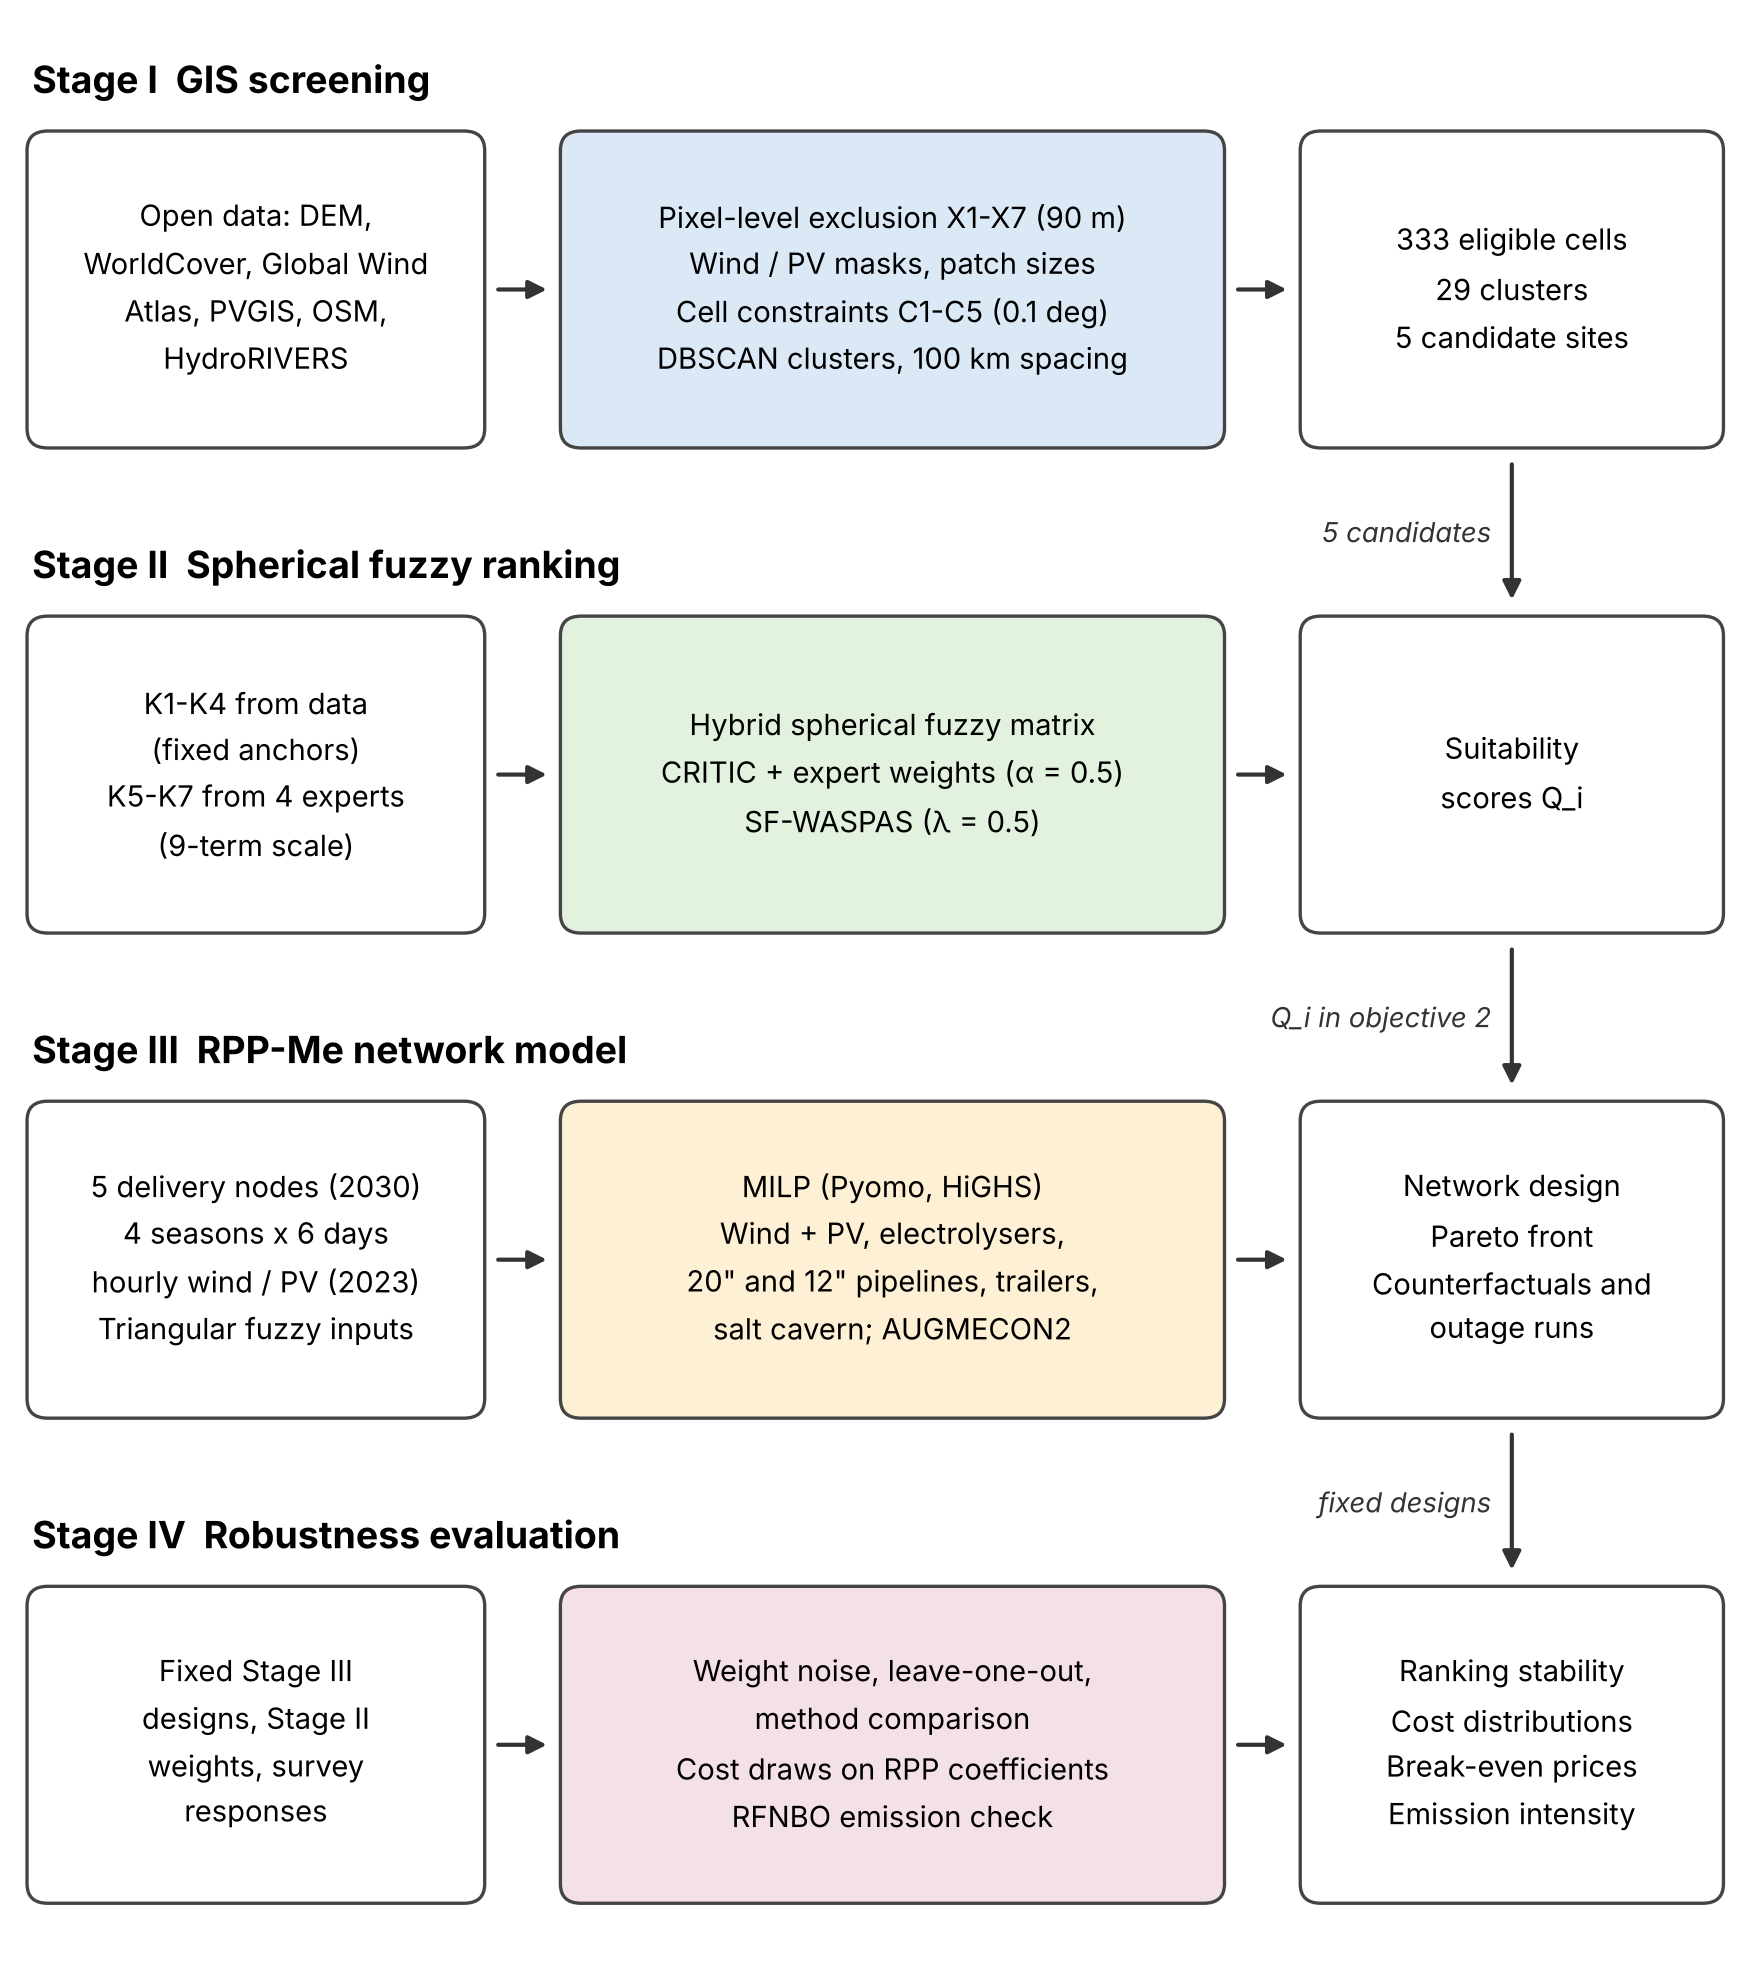
\includegraphics[width=0.88\textwidth]{Fig0_method_overview.png}
\caption{Overview of the four-stage framework. Stage~I yields candidate sites, Stage~II their suitability scores $Q_i$, Stage~III the network design and cost--suitability Pareto front, and Stage~IV tests the ranking and fixed designs.}
\label{fig:method}
\end{figure}

\subsection{Stage I --- GIS-Based Exclusion and Candidate Generation}
Stage~I screens the whole of Türkiye for land on which a hybrid wind--photovoltaic (PV) plant with co-located electrolysis could be developed. The exclusion buffers reported in the siting literature (0.1--5\,km) are smaller than a $0.1^\circ$ cell, which measures about 92--100\,km$^2$ between 36 and 42$^\circ$N, so applying them to whole cells would be either ineffective or excessively strict. Following land-eligibility practice \citep{ryberg2018uniformly,pfennig2023global,ishmam2024mapping}, exclusions are therefore applied at the pixel level (3\,arcsec, $\approx$90\,m), and the remaining eligible area is aggregated to the cell. Supplementary Table~S8 lists the criteria in three groups: common exclusions (X1--X7) of land unavailable to any technology; technology masks, under which wind pixels need a slope of at most 30\% and a gross capacity factor (CF) of at least 25\% while PV and electrolyser pixels need a slope of at most 10\% and must lie outside the cropland that Turkish soil-protection law reserves for agriculture; and cell-level constraints (C1--C5) on solar irradiation, eligible area, and reach to freshwater or coastline and to a high-voltage substation. Within each mask only contiguous patches (8-connectivity) are retained, at least 10\,km$^2$ for wind \citep{pfennig2023global} and 3\,km$^2$ for PV, the latter corresponding to $\approx$100\,MW$_\text{ac}$ at the 31\,MW$_\text{ac}$/km$^2$ total-area density of large PV plants \citep{ong2013land}.

The wind threshold refers to the gross CF of the Global Wind Atlas, which excludes wake and other losses \citep{davis2023global}. With the 20\% loss allowance of \citet{lu2009global}, a gross CF of 25\% corresponds to a net CF of about 20\%. This is below the Turkish fleet average of 30\% for 2006--2020 \citep{kursun2022}, so the threshold acts as a conservative technical floor rather than a profitability criterion.


Suitable cells are grouped into spatially contiguous clusters by density-based spatial clustering of applications with noise (DBSCAN; \citealp{ester1996density}; $\varepsilon = 0.15^\circ$, which links diagonal neighbours; minimum of three cells). Clusters are ranked by their total wind- and PV-eligible area. This objective measure of buildable potential leaves all preference judgements to Stage~II. Each cluster is represented by its cell with the largest eligible area. Clusters are taken in rank order until five candidates are selected. A cluster is skipped if its representative cell lies within 100\,km of a candidate already selected. The rule spreads the candidates over distinct resource regimes, which is the basis of a resilient supply portfolio. Wind farms less than about 50\,km apart produce highly correlated output, whereas the correlation halves at around 200\,km \citep{katzenstein2010variability}; the 100\,km threshold lies at the lower end of the wind correlation lengths of 89--447\,km reported by \citet{stmartin2015variability}.

All spatial inputs are checksum-frozen open datasets covering boundaries, terrain, land cover, wind and solar resources, hydrography and infrastructure \citep{runfola2020geoboundaries,copernicusdem,zanaga2022worldcover,davis2023global,huld2012pvgis,pfeifroth2024sarah3,lehner2013hydrorivers,naturalearth,osm2026}; Supplementary Table~S8 names the dataset behind each criterion.

An extraction step computes all cell-level attributes once into a frozen feature table, with snapshots of the OpenStreetMap layers and the source URLs and 256-bit Secure Hash Algorithm (SHA-256) checksums of all inputs; a deterministic selection step then derives the eligible cells, clusters and candidates from that table alone, making the threshold sensitivity analysis of Section~\ref{sec:gis_results} exactly repeatable without network access.

\subsection{Stage II --- Spherical Fuzzy CRITIC--WASPAS with a Hybrid Decision Matrix}
\label{sec:stage2_method}

\subsubsection{Criteria selection}
The preference criteria were selected by a documented procedure rather than adopted from a single precedent. Twenty-two green hydrogen production, hub and storage siting studies were coded for the criteria they use, following the approach of recent siting reviews \citep{zun2026review,pinedaserna2023}; synonymous criteria were then harmonised and screened by how often they recur. The coded set, the criterion-frequency matrix on which the screening rests, and the criteria that were considered and not retained are given in Supplementary Table~S3. Renewable resource, transport access, terrain, water, grid connection and protected areas recur throughout this literature, while social acceptance, water stress, natural hazard and policy criteria are increasingly emphasised \citep{zun2026review,tonelli2023global}. Each surviving criterion was then assigned to a single decision role, and was retained only where it is measurable from a documented dataset or can be anchored for expert judgement, and where it discriminates among the candidates at this scale.

Two rules govern role assignment. First, quantities optimised in Stage~III (production cost, transport cost and CO$_2$ abatement) are excluded from Stage~II, since including them would count the same economic information twice once Stage~II scores enter the Stage~III objective \citep{zun2026review}. Second, a variable already used as a hard constraint in Stage~I is reused only if it varies materially among the candidates above the threshold or measures a different construct, as water stress does relative to distance to water. Geological hydrogen storage, rarely a production-siting criterion and concentrated in a single Turkish geography (the Tuz Gölü salt caverns; \citealp{ozarslan2012}), enters Stage~III as a candidate storage node rather than as a siting criterion \citep{raeesi2023}.

The procedure yields seven criteria (Supplementary Table~S9). Four are computed from open data and three are elicited from experts.


\subsubsection{Hybrid spherical fuzzy decision matrix}
A spherical fuzzy number (SFN) $\tilde{s} = (\mu, \nu, \pi)$ carries membership, non-membership and hesitancy degrees in $[0,1]$ with $\mu^2 + \nu^2 + \pi^2 \le 1$ \citep{gundogdu2019spherical}. Supplementary Note~S12 gives its score function, the CRITIC weights and the WASPAS aggregation; the score runs from $-0.64$ to $0.64$ along the nine linguistic terms, and every aggregated expert entry was checked for sign consistency against $\mu-\nu$.

\textit{Expert-judged criteria.} Experts rate criteria K5--K7 on the nine-term linguistic scale of \citet{kutlugundogdu2019waspas}, adopted verbatim. The scale runs from absolutely low $(0.1, 0.9, 0.1)$ through equal $(0.5, 0.5, 0.5)$ to absolutely high $(0.9, 0.1, 0.1)$. A ``no basis to judge'' option is treated as missing rather than as a neutral rating. Individual judgements are aggregated with the spherical weighted arithmetic mean (SWAM) \citep{kutlugundogdu2019waspas}.

\textit{Data-derived criteria.} Criteria K1--K4 are normalised against fixed anchors $L_j$ and $U_j$ that do not depend on the five candidates. Benefit criteria use $r_{ij} = (x_{ij} - L_j)/(U_j - L_j)$ and cost criteria use $r_{ij} = (U_j - x_{ij})/(U_j - L_j)$, with $r_{ij}$ clipped to $[0,1]$. Where a published scale or a Stage~I threshold exists, it defines the anchors: 0--50\,km for K1 (the Stage~I substation radius) and 0--5 for K2 (the Aqueduct score scale). Otherwise the anchors are the 5th and 95th percentiles over all 333 Stage~I-eligible cells: 8.4--82.2\,km for K3 and 0.078--0.332\,g for K4. Fixed anchors avoid inflating small differences among only five candidates, as min--max normalisation would. Measured values carry no hesitancy, so they become SFNs with $\pi = 0$ \citep{sharaf2023}. They are mapped as $(0.18 + 0.64 r_{ij},\, 0.82 - 0.64 r_{ij},\, 0)$, which keeps $\mu+\nu=1$ and gives a score of $1.28\,r_{ij}-0.64$: the same range, $\pm0.64$, as the nine linguistic terms. Measured data can therefore be no more extreme than the strongest expert judgement, and the mapping avoids the zero membership that would act as a veto in the geometric aggregation below. (Mapping membership onto $[0.1,0.9]$ with $\pi=0$ would instead give data scores of $\pm0.80$, wider than any linguistic term, and inflate the data criteria's contrast.) Comparable hybrid matrices have been used in recent hydrogen-siting studies \citep{du2025site,ali2026optimal}.


\subsubsection{Combined subjective--objective weights}
CRITIC derives objective weights from the contrast and conflict of the criteria in the decision matrix \citep{diakoulaki1995determining}; as in the original method, each column of the defuzzified matrix is first rescaled to $[0,1]$ by its own minimum and maximum, so that a criterion's weight reflects its relative contrast rather than the spread of its measurement scale (Supplementary Note~S12).
With only five alternatives, each correlation coefficient rests on five observations, and CRITIC does not reflect decision relevance. Experts therefore also rate the importance of all seven criteria on the same scale. The aggregated importance SFNs are defuzzified with the same score function. Because the score can be negative, the subjective weights are $w_j^{S} = (1 + \text{Score}_j)/\sum_l (1 + \text{Score}_l)$. The final weights are the convex combination \citep{ma1999,wu2021site}
\begin{equation}
w_j = \beta\, w_j^{S} + (1 - \beta)\, w_j^{C}, \qquad \beta = 0.5 ,
\end{equation}
with $\beta$ held at 0.5 throughout.

\subsubsection{Spherical-Fuzzy WASPAS}
Following \citet{kutlugundogdu2019waspas}, the suitability score $Q_i$ combines the scores of the weighted sum and weighted product models, computed in spherical fuzzy arithmetic with the spherical weighted arithmetic and geometric means (Supplementary Note~S12).
For use as a coefficient in Stage~III, $Q_i$ is rescaled to $Q_i^{01} = (1 + Q_i)/2$.

\subsection{Stage III --- Seasonal Robust Possibilistic Network Model}

\textit{Network and time structure.} The network connects the five Stage~I candidates $i \in I$, the baseline demand nodes $j \in J$ (Supplementary Table~S1) and the Tuz Gölü salt-cavern storage node $g$. Facilities less than 2\,km apart share a delivery point, so the seven baseline facilities form five nodes: the İzmir (Aliağa) and STAR refineries, and the İzmit refinery and the İGSAŞ ammonia complex, are each served by one connection, at the Aliağa and Körfez hubs; Gemlik, Kırıkkale and Batman are the remaining nodes. Arcs run from sites to demand nodes, from sites to storage and from storage to demand nodes. Their lengths $L_a$ are Open Source Routing Machine (OSRM) road distances \citep{luxen2011real}. Each arc can carry a new hydrogen pipeline of one of two diameter classes, 20-inch (1.2\,GW, 864\,t/d; \citealp{ehb2022}) or 12-inch (222\,t/d, with capacity and cost extrapolated from the European Hydrogen Backbone classes; Supplementary Table~S2, Note~N12), and compressed hydrogen in tube trailers. Trailer costs are levelised and distance-dependent \citep{desnz2023transport}; above about 400\,km, where a trailer can no longer complete the roughly 300 round trips a year assumed by the levelised costs, the additional trailer capital is added explicitly (Supplementary Table~S2, Note~N13). Trailers leaving the cavern are refilled to 500\,bar on grid electricity (Supplementary Table~S2, Note~N14).

The year is represented by four seasons of six representative days of 24 hours, selected by $k$-medoids clustering \citep{kotzur2018impact} from hourly 2023 profiles and rescaled so that the weighted profiles reproduce each technology's annual energy; day weights $w_d$ sum to 365. Wind profiles come from 100\,m wind speeds in the fifth-generation reanalysis of the European Centre for Medium-Range Weather Forecasts (ERA5) \citep{hersbach2020era5}, scaled to the Global Wind Atlas gross capacity factor and converted with the power curve of the Vestas V126-3.45\,MW, the turbine the Global Wind Atlas itself uses for IEC Class~II \citep{davis2023global,windpowerlib2024}. PV profiles are the PVGIS-SARAH3 output of a fixed, optimally tilted system with 14\% losses \citep{huld2012pvgis}.

\textit{Electricity source.} The electrolysers are supplied only by new, unsupported wind and PV plants co-located with them, which satisfies the additionality and correlation rules for renewable hydrogen (RFNBO) in Delegated Regulation (EU) 2023/1184, including the hourly temporal correlation that applies from 2030 \citep{eu2023da1184}. Grid electricity is not used for electrolysis: at Türkiye's 2023 grid emission factor \citep{menr2025ef} it would emit about seven times the RFNBO threshold \citep{eu2023da1185}. The grid connection therefore serves only to sell surplus electricity, and its capacity is limited to the electrolyser capacity. Renewable capacity is limited by the eligible area of the candidate's 0.1$^{\circ}$ cell, at 3.0\,MW/km$^2$ for wind \citep{denholm2009land} and 31\,MW/km$^2$ for PV \citep{ong2013land}.

The land constraint accounts for the measured intersection and union of the two eligible-area masks; $\phi\in\{0,0.5,1\}$ specifies the share of their overlap available for co-use. The baseline uses full measured co-use ($\phi=1$).

Hourly renewable generation supplies electrolysis, compression and exports; any remainder is curtailed. Hydrogen is dispatched by pipeline or tube trailer. The baseline uses 55\,kWh/kg for electrolysis \citep{doe2024record} and compression requirements of 0.56\,kWh/kg for pipeline injection and 2.41\,kWh/kg for 500-bar trailer filling \citep{desnz2023transport}.

Demand nodes receive constant daily quantities, and pipeline flows are bounded by the binary construction decision. Seasonal cavern inventory is tracked at season boundaries with cyclic year-end closure. Injection and withdrawal are limited to 1,860 and 2,481\,t/d, derived from natural-gas design rates; working gas is capped at 62,013\,t for the twelve existing caverns \citep{san2019tuz}. The cap is conservative given the expansion from 1.2 to 5.4\,bcm of natural-gas capacity \citep{aiib2018tuzgolu}. Depleted Silivri storage is excluded because its higher cushion-gas requirement and contamination risk make it less suitable than salt caverns \citep{baki2022botas}. Site opening requires at least 50\,MW of electrolysis capacity \citep{menr2023hydrogen}.

\textit{Uncertain parameters.} All cost parameters and demand are triangular fuzzy numbers $\tilde{c} = (c_1, c_2, c_3)$; their values, sources and derivations are reported in Supplementary Table~S2. The principal cost ranges draw on the International Renewable Energy Agency (IRENA), the International Energy Agency (IEA), the European Hydrogen Observatory and salt-cavern cost data \citep{irena2025costs,iea2024global,eho2025,papadias2021bulk}. Demand is $\tilde{d}_j = \sum_{n\in N_j}\tilde{\theta}_{\sigma(n)}\, D_n$, where $D_n$ is the on-purpose hydrogen consumption of facility $n$ at node $j$ and $\tilde{\theta}_{\sigma(n)}$ is the renewable share of its sector derived in Section~\ref{sec:demand}. Türkiye is not bound by the RFNBO targets behind $\tilde{\theta}$, but they are the relevant benchmark for export-oriented producers.

Annualised unit costs are monotone in capital expenditure (CAPEX), the weighted average cost of capital (WACC), lifetime and operation and maintenance (O\&M). Their vertices are therefore obtained from the extreme values; for example, using the capital recovery factor (CRF), the lower vertex is $\text{CAPEX}_1\,\text{CRF}(r_1, n_3) + \text{O\&M}_1$. Technical coefficients ($\eta$, compression energies) are held at their modal values and varied in the sensitivity analysis.

{\itshape Uncertainty and objective.} The Me measure combines possibility and necessity, with $\lambda$ controlling the decision attitude \citep{xu2013approximation}; at $\lambda=0.5$, its expected value coincides with \citet{jimenez2007linear}. Robust possibilistic programming makes each demand confidence level a decision variable \citep{pishvaee2012robust}. The objective combines Me-expected annual cost, export revenue at the day-ahead price \citep{epias2024}, a range penalty weighted by $\gamma=0.2$, and a penalty $\delta$ on possible demand violation, priced at the import parity of each facility's sector: 5.63\,€/kg for the ammonia plants, which can import renewable ammonia \citep{h2global2024}, and 7.30\,€/kg for the refineries, which need cracked hydrogen \citep{spglobal2025cracking}. The baseline uses $\lambda=0.5$. Because the Me constraint is used on its $\alpha_j\ge\lambda$ branch, the modal demand is always supplied domestically; this is stated as an explicit security-of-supply mandate, and an import diagnostic in which imports at parity may replace any part of the demand shows what the mandate costs. The full algebraic model, including the expected-cost calculation, the constraints and the unit conventions, is given in Supplementary Note~S7.
The model has about 19,600 variables, including 52 binaries. It is implemented in Pyomo \citep{bynum2021pyomo} and solved with HiGHS \citep{huangfu2018parallelizing} to a relative mixed-integer programming (MIP) gap of 0.1\%.

Sensitivity and counterfactual runs (Sections~\ref{sec:stage3_base}--\ref{sec:rfnbo}) vary the land basis (cluster instead of cell, reported as a second baseline), the co-use share $\phi$, the electrolyser consumption $\eta$ (48 and 57.5\,kWh/kg), the trailer operating hours, the demand basis, and $\gamma$, $\delta$ and $\lambda$. They also evaluate a stepwise decomposition of the logistics result from a reference configuration (single demand share, separate nodes, one diameter, no long-haul or cavern-refill terms), a sequential counterfactual in which the ranking pre-filters to the three highest-ranked candidates before cost-only optimisation, and a deterministic design at modal values with $\gamma=0$. Two electricity configurations are tested: S-island, with no surplus sales; and S-grid, which allows grid import under annual matching against exports, as in Türkiye's Renewable Energy Resource Guarantee Certificate (YEK-G) system. Under S-grid each site has an hourly import variable $im_{idh}$ whose weighted annual total may not exceed the weighted annual export; grid electricity for cavern injection and pipeline recompression is accounted separately.

\subsection{Linking Stages II and III}
 Stage~II supplies the non-monetary suitability scores $Q_i$; Stage~III balances robust cost against the suitability of the sites where hydrogen is produced. Production weighting avoids rewarding either site openings alone or output volume. We trace the Pareto front with the augmented $\varepsilon$-constraint method 2 (AUGMECON2), using the linear reformulation of the suitability constraint and a normalised slack \citep{mavrotas2009effective,mavrotas2013improved}. This follows network-design studies that optimise stakeholder preferences alongside cost \citep{becker2023integrated,olabi2026dynamic}.

\subsection{Stage IV --- Monte Carlo Robustness Evaluation}
Stage~IV evaluates both upstream stages by simulation ($N = 10{,}000$, fixed seed). It is an out-of-sample robustness evaluation under sampled parameters, not a validation against observed data.
\begin{enumerate}
    \item \textit{Ranking stability (Stage~II).} Following the sensitivity logic of \citet{triantaphyllou1997sensitivity}, the criteria weights are perturbed as $w_j' = w_j(1 + \sigma\varepsilon_j)$ with $\varepsilon_j \sim N(0,1)$ and relative noise levels $\sigma \in \{0.05, 0.10, 0.15, 0.20\}$, then renormalised. The stability index (SI) is the share of draws in which the top-ranked site keeps first place; the rank preservation ratio (RPR) is the share in which the whole ranking is unchanged. Because these indices are uninformative when one alternative dominates on several criteria, leave-one-criterion-out and a comparison of six ranking methods are reported as well.
    \item \textit{Design robustness (Stage~III).} The capacities and flows of a Stage~III design are fixed; there is no re-dispatch. Each annualised cost coefficient of the RPP objective is sampled independently from its own triangular distribution, a probabilistic reading of the same possibility distribution that the RPP uses; sampling the underlying CAPEX, WACC and lifetime separately is reported as a secondary reading. One common uniform draw is mapped to every facility's demand through the inverse distribution function of its sector's triangle. Unmet demand is valued at the facility's import parity. The shortfall probability is reported for the system (total demand above total delivery) and for any node. Designs are compared using common random numbers, and break-even import prices are computed at which a hedged design and the baseline have equal mean total cost.
    \item \textit{Emission check.} Electrolysis is supplied by co-located new renewable plants and therefore carries no electricity emissions, so only logistics emissions count against the RFNBO threshold. These are evaluated for each design from the grid electricity used for cavern injection, trailer refilling at the cavern and pipeline recompression, and from trailer diesel, at the factors given in Section~\ref{sec:rfnbo} and for trailer payloads of 300, 1,000 and 1,300\,kg.
\end{enumerate}

\section{Case Study --- Türkiye: Demand Basis and Stage I Results}

The national strategy sets electrolyser targets but no tonnage targets for hydrogen use \citep{menr2023hydrogen}, so the 2030 demand is derived in Section~\ref{sec:demand}.

\subsection{Stage I Results --- Eligible Land and Candidate Sites}
\label{sec:gis_results}
Supplementary Table~S4a traces the pixel-level exclusions across Türkiye's 776,243\,km$^2$ of land; the common exclusions leave 300,541\,km$^2$ (38.7\%). Built-up areas with their 1\,km buffer (218,128\,km$^2$) and tree cover with permanent snow and ice (194,083\,km$^2$) account for most of the reduction, which agrees with the finding of \citet{ryberg2018uniformly} that settlement setbacks are among the most land-intensive constraints. Among the technology criteria, the wind resource is the most selective: a gross CF of at least 25\% on buildable, sufficiently flat land is met on 52,114\,km$^2$ (6.7\%), of which 35,132\,km$^2$ (4.5\%) forms contiguous patches of at least 10\,km$^2$. For PV and electrolysis, the exclusion of cropland reduces flat buildable land from 149,681 to 52,305\,km$^2$, and contiguous patches of at least 3\,km$^2$ cover 19,089\,km$^2$ (2.5\%).

At the cell level, 333 of the 8,115 cells (4.1\%) satisfy all five constraints (Supplementary Table~S4b; Fig.~\ref{fig:gis_filter_results}). The binding constraints are the wind- and PV-eligible areas. Solar irradiation removes only the humid Black Sea fringe (711 cells). The water and substation constraints are not binding at the national scale: every cell lies within 50\,km of a perennial river, a freshwater lake or the coast, and 8,102 cells lie within 50\,km of a $\ge$154\,kV substation. Both constraints are retained as safeguards, and grid proximity re-enters Stage~II as a continuous preference (K1).

\begin{figure}[htbp]
\centering
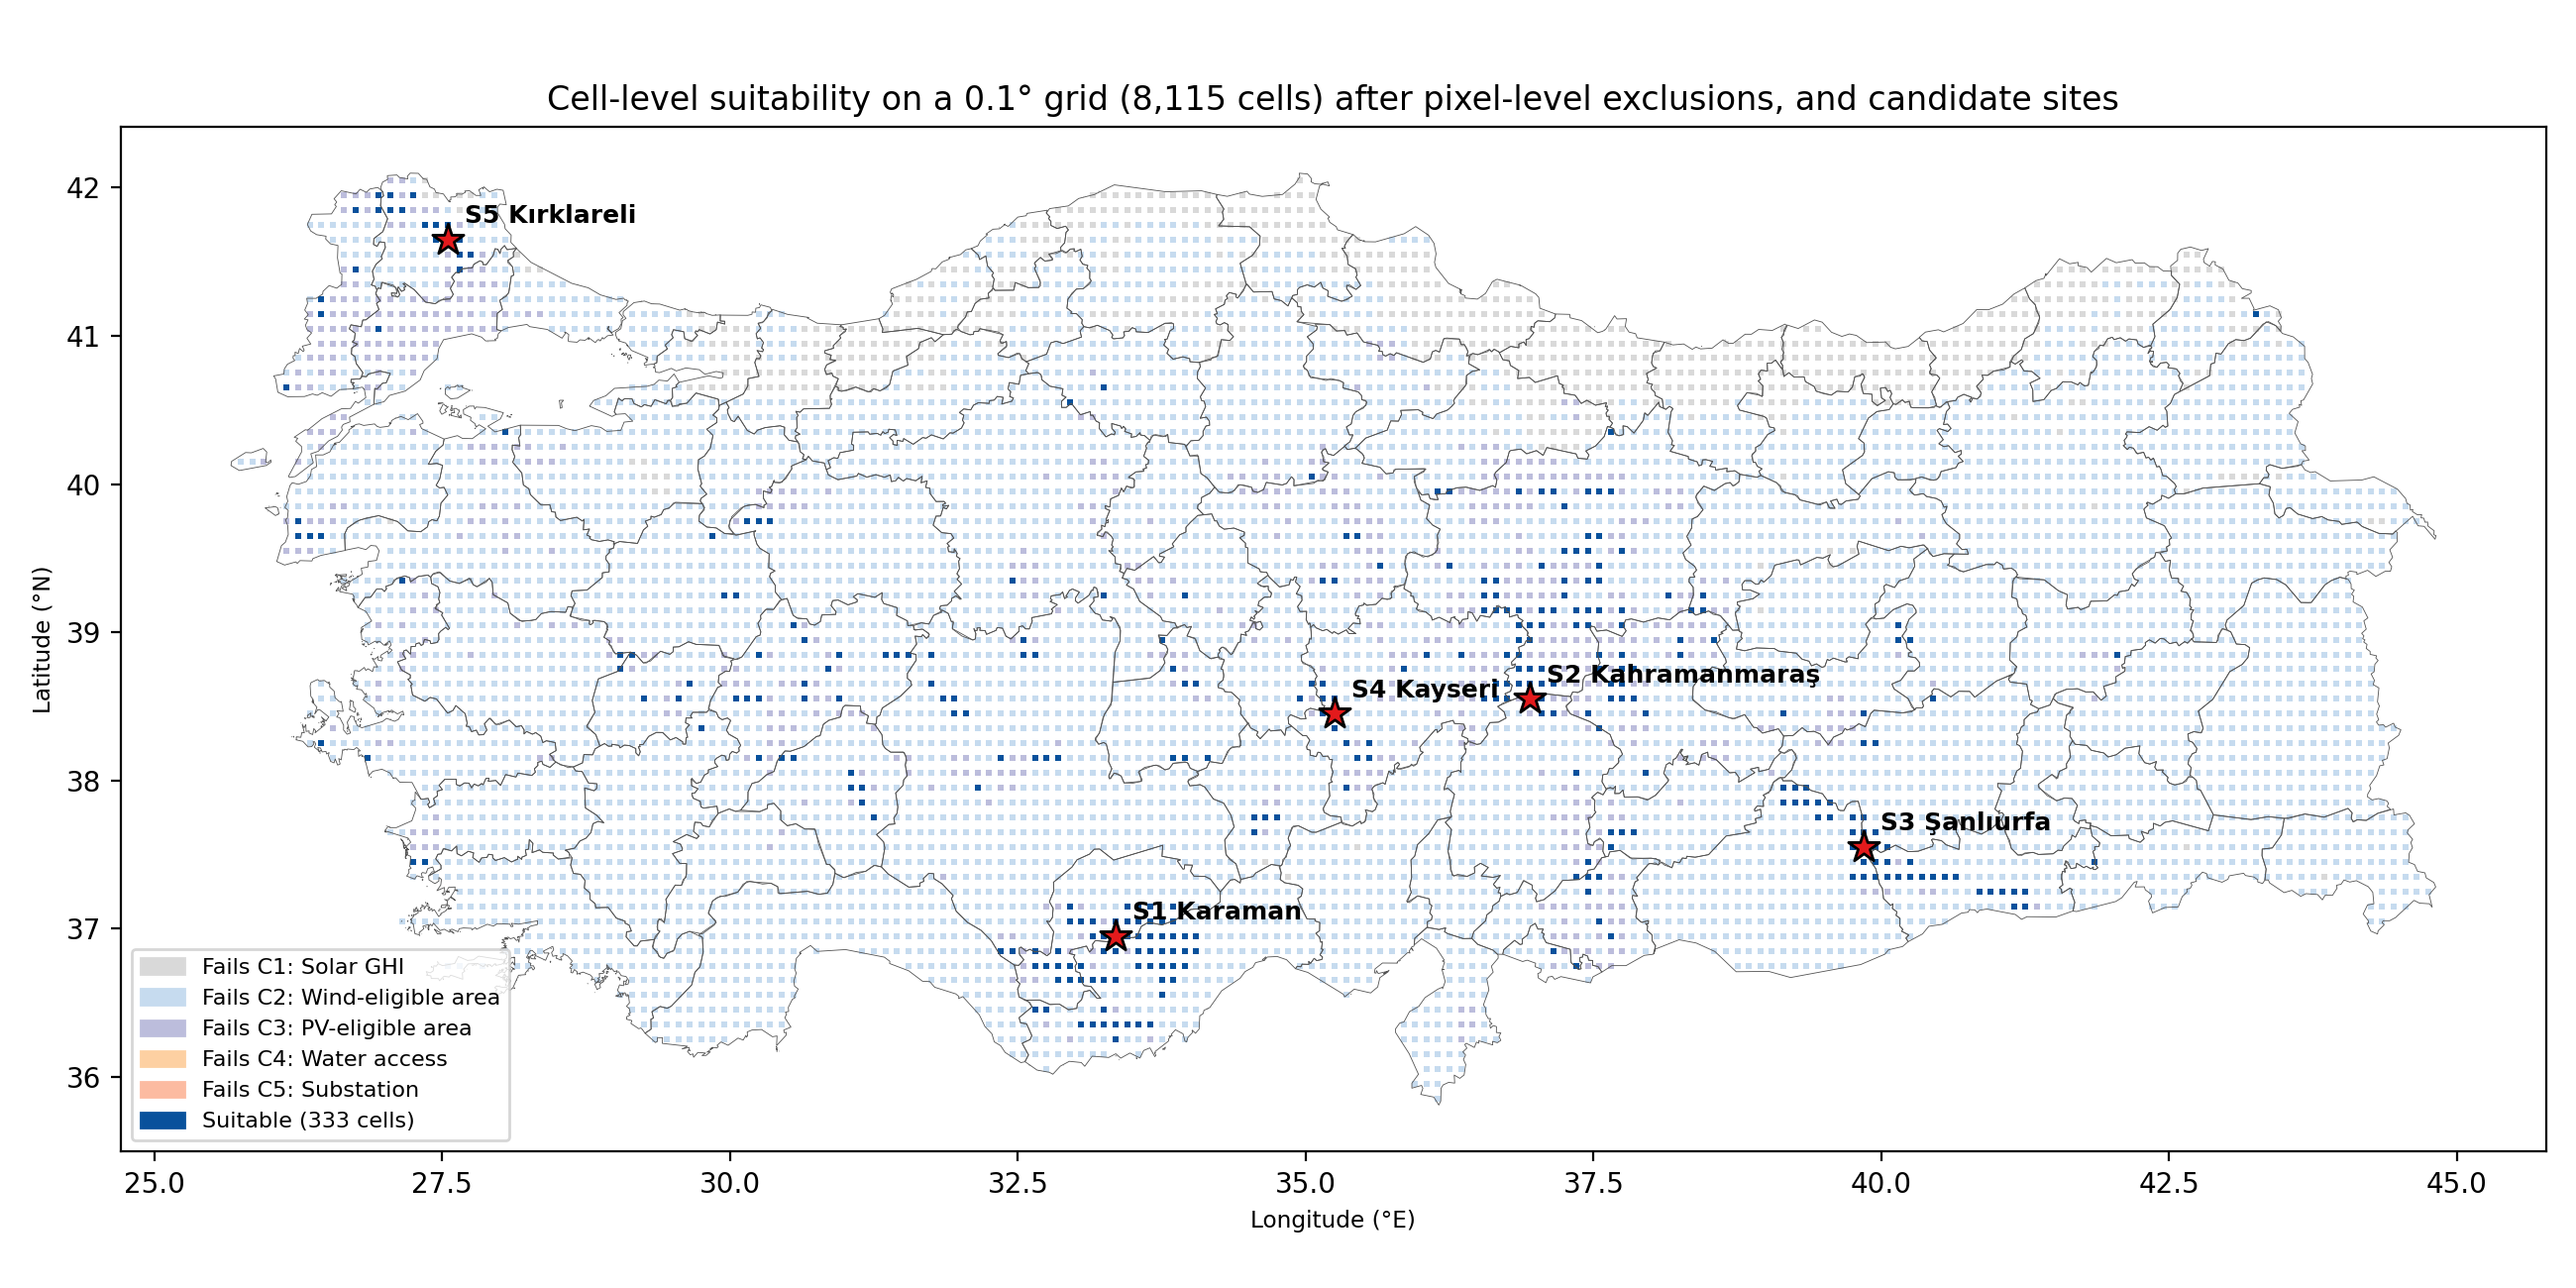
\includegraphics[width=\textwidth]{Fig1_GIS_filter_results.png}
\caption{Cell-level suitability after pixel-level exclusions. Cells are coloured by the first constraint they fail; suitable cells are dark blue and the five candidate sites are marked with stars.}
\label{fig:gis_filter_results}
\end{figure}

The 333 suitable cells form 29 clusters. A 100\,km spacing rule selects five candidates (Table~\ref{tab:candidate_sites}): S1--S4 on interior plateaus at 1,080--1,840\,m and S5 in Thrace at 315\,m. S5 alone lies within 300\,km by road of Marmara (Supplementary Table~S1). Eligible areas are mainly grassland, shrubland or bare land; each candidate is within 22\,km of a high-voltage substation and 13\,km of perennial freshwater.

\begin{table}[htbp]
\centering
\caption{Stage~I candidate sites. Cluster values refer to the whole DBSCAN cluster; site values refer to its representative cell (largest eligible area).}
\label{tab:candidate_sites}
\resizebox{\textwidth}{!}{%
\begin{tabular}{lllrrrrrrrr}
\toprule
 & & & & \multicolumn{3}{c}{Cluster} & \multicolumn{4}{c}{Representative cell} \\
\cmidrule(lr){5-7}\cmidrule(lr){8-11}
Site & Province (district) & Lat, Lon & Cells & Wind area & PV area & Total & Gross CF & GHI & Elevation & Substation \\
 & & ($^\circ$N, $^\circ$E) & & (km$^2$) & (km$^2$) & (km$^2$) & (\%) & (kWh/m$^2$) & (m) & (km) \\
\midrule
S1 & Karaman & 36.95, 33.35 & 40 & 2,388 & 1,325 & 3,713 & 34.1 & 1,801 & 1,612 & 11.8 \\
S2 & Kahramanmaraş (Afşin) & 38.55, 36.95 & 40 & 1,802 & 442 & 2,244 & 33.6 & 1,780 & 1,839 & 21.7 \\
S3 & Şanlıurfa (Viranşehir) & 37.55, 39.85 & 23 & 962 & 700 & 1,662 & 27.1 & 1,830 & 1,356 & 13.4 \\
S4 & Kayseri (Develi) & 38.45, 35.25 & 12 & 538 & 272 & 810 & 28.7 & 1,788 & 1,080 & 5.4 \\
S5 & Kırklareli (Pınarhisar) & 41.65, 27.55 & 9 & 375 & 98 & 473 & 33.7 & 1,544 & 315 & 4.0 \\
\bottomrule
\end{tabular}%
}
\end{table}

Supplementary Table~S4c reports the sensitivity of the candidate set to the main thresholds and to the spacing rule: S1 and S3 are selected in all twelve scenarios and S2 in ten; the gross CF threshold and the cropland exclusion are the most influential assumptions; the water and substation thresholds have almost no effect; and the spacing rule changes only which of the lower-ranked candidates is selected.

\subsection{Industrial Hydrogen Demand Nodes}
\label{sec:demand}
Demand nodes were defined independently of the candidate sites. The inventory covers 20 Turkish facilities that produce or consume hydrogen, or have announced plans to do so (Supplementary Table~S1); the baseline retains the seven operating sites with on-site hydrogen use of at least 1\,kt/yr --- five refineries and two ammonia complexes --- while a 2040 scenario adds two integrated steelworks planning hydrogen-based direct reduction (H$_2$-DRI). Imported-ammonia plants, by-product hydrogen users and projects without quantified demand are excluded.

Because neither official statistics \citep{tuncer2026enerji} nor operators report hydrogen consumption, demand is estimated from published production capacities (Supplementary Table~S1): refineries at the EU-average 9.6\,kg\,H$_2$/t crude capacity, of which about 60\% (5.5\,kg/t) comes from dedicated reformers and can be directly substituted \citep{catf2025hydrogen}; ammonia at 0.1776\,t\,H$_2$/t NH$_3$; and H$_2$-DRI at 47--57\,kg\,H$_2$/t DRI \citep{vogl2018assessment,rechberger2020green}. The average refinery intensity may understate complex refineries such as İzmit and STAR and overstate the simple Batman refinery.

On-purpose hydrogen demand at the seven baseline facilities is estimated at 0.38\,Mt/yr (0.55\,Mt/yr including by-product hydrogen): 237\,kt/yr at the five refineries and 139\,kt/yr at the two ammonia complexes, concentrated in Marmara and the Aegean, with Kırıkkale and Batman as inland nodes. Facility-level values are in Supplementary Table~S1.

The renewable share differs by sector because the revised Renewable Energy Directive (RED III) treats the two uses differently \citep{eu2023red3}. For ammonia the industry target applies: $\tilde{\theta}_{\mathrm{NH_3}} = (0.336, 0.42, 0.60)$, the 2030 target of 42\%, its reduced alternative and the 2035 target of 60\%. Refinery hydrogen is excluded from that target and counts instead towards the transport sub-target, which requires at least one percentage point of RFNBOs in 2030 at double counting \citep{h2europe2024red3,cho2026red}; applied to Türkiye's 2024 transport final energy excluding aviation \citep[1,125\,PJ;][]{tuik2026transport} this gives $\tilde{\theta}_{\mathrm{ref}} = (0.158, 0.198, 0.395)$ of refinery on-purpose demand and bounds the refinery role from above (Supplementary Table~S2, Note~N11). The resulting modal renewable demand is 105.2\,kt/yr, with a possibility range of 84.2--177.1\,kt/yr; applying the industry share to all facilities, as an upper-bound scenario, gives 157.9\,kt/yr.

\section{Results and Discussion}
All numbers in this section are produced by the scripts in the repository (see Data Availability). All Stage~III solutions were solved to a relative MIP gap of at most 0.1\%.

\subsection{Stage II --- Siting Rankings from the Hybrid Spherical-Fuzzy CRITIC--WASPAS Framework}
\label{sec:stage2_results}
The nine-term spherical-fuzzy survey combined direct importance ratings from four senior specialists (two public-sector permitting and EIA experts and two renewable-energy academics) with CRITIC contrast weights at $\beta=0.5$ (Table~\ref{tab:stage2_results}). The combined weights are close to uniform (0.121--0.178): seismic hazard receives the largest weight, and the four data-derived criteria together carry 0.59. The expert ratings of the three judged criteria lie close to neutral ($p$ = 0.49--0.59), so these criteria discriminate little among the candidates.

The ranking is S5 $>$ S4 $>$ S2 $>$ S3 $>$ S1: Kırklareli first, then Kayseri, Kahramanmaraş, Şanlıurfa and Karaman. Its lead comes mainly from measured data: basin water stress (2.09 against 4.86--5.00 for the interior sites) and close grid access, reinforced by the panel's strongest logistics-ecosystem rating. The $Q^{01}$ scores span only 0.504--0.568.

Five checks bound this result. Leave-one-criterion-out leaves S5 first in all seven cases, but removing water stress narrows its lead over the second site from 0.040 to 0.010, so the separation rests largely on one criterion. Six ranking variants that differ in the data mapping, the CRITIC normalisation and the use of fuzzy arithmetic (Supplementary Table~S5) all place S5 first and S1 last, while S2--S4 change places. Under Monte Carlo weight perturbation ($N = 10{,}000$), S5 keeps first place in every draw at relative noise levels of 5--20\% ($\text{SI} = 1.000$), while the rank preservation ratio of the full ordering falls from 1.000 at 5\% to 0.830 at 20\%; omitting each respondent in turn leaves S5 first. Replacing the GEM values of K4 with those of the national AFAD hazard map at the same coordinates leaves the ordering unchanged, narrowing S5's lead over S4 from 0.040 to 0.023. Varying $\beta$ from 0 to 1 leaves the ranking unchanged, and S5's lead over S4 is widest under pure CRITIC weights (Supplementary Table~S13), so it rests on data rather than judgement. These checks cover weights, criteria, single respondents and the hazard source.

\begin{table}[htbp]
\centering
\caption{Stage~II hybrid decision matrix, criteria weights, and spherical fuzzy WASPAS suitability scores ($w_j = 0.5\,w_j^S + 0.5\,w_j^C$). K1--K4 are raw values; K5--K7 are defuzzified panel ratings.}
\label{tab:stage2_results}
\small
\resizebox{\textwidth}{!}{%
\begin{tabular}{lrrrrrrrrrrr}
\toprule
Site & K1 Substation & K2 Water & K3 Protected & K4 PGA & K5 Social & K6 Permitting & K7 Logistics & Score & Score & $Q$ & $Q^{01}$ (rank) \\
 & (km) & (0--5) & (km) & (g) & ($p_{i5}$) & ($p_{i6}$) & ($p_{i7}$) & WSM & WPM & & \\
\midrule
S1 Karaman & 11.8 & 5.00 & 18.0 & 0.093 & 0.518 & 0.497 & 0.528 & 0.071 & $-0.053$ & 0.009 & 0.504 (5) \\
S2 Kahramanmaraş & 21.7 & 4.86 & 39.6 & 0.129 & 0.576 & 0.507 & 0.569 & 0.085 & 0.008 & 0.047 & 0.523 (3) \\
S3 Şanlıurfa & 13.4 & 5.00 & 44.7 & 0.092 & 0.526 & 0.492 & 0.513 & 0.085 & $-0.013$ & 0.036 & 0.518 (4) \\
S4 Kayseri & 5.4 & 5.00 & 34.6 & 0.156 & 0.544 & 0.524 & 0.569 & 0.105 & 0.009 & 0.057 & 0.528 (2) \\
S5 Kırklareli & 4.0 & 2.09 & 30.5 & 0.092 & 0.524 & 0.507 & 0.592 & 0.169 & 0.105 & 0.137 & 0.568 (1) \\
\midrule
$w_{\text{CRITIC}}$ & 0.136 & 0.127 & 0.143 & 0.211 & 0.153 & 0.121 & 0.108 & & & & \\
$w_{\text{expert}}$ & 0.154 & 0.133 & 0.134 & 0.145 & 0.134 & 0.166 & 0.134 & & & & \\
$w_{\text{final}}$ & 0.145 & 0.130 & 0.139 & 0.178 & 0.144 & 0.144 & 0.121 & & & & \\
\bottomrule
\end{tabular}%
}
\end{table}

\subsection{Stage III --- Baseline Network Design}
\label{sec:stage3_base}
In the baseline ($\lambda = 0.5$, $\gamma = 0.2$, sector-specific import parity), the network delivers 105.2\,kt\,H$_2$/yr, the modal renewable demand. The expected total annual cost $E_{\text{Me}}[z]$ corresponds to a delivered cost of 9.96\,€/kg, i.e. the levelised cost of hydrogen delivered to the demand nodes, which is the per-kilogram measure reported throughout and is not comparable with plant-gate LCOH. Four of the five candidates are opened; Şanlıurfa (S3), the most remote from the Marmara and Aegean demand, is not (Table~\ref{tab:stage3_sites}, Fig.~\ref{fig:network}).

Land binds at Karaman (S1) and Kırklareli (S5), where both wind and PV reach the eligible area of the candidate cell, and wind binds at Kahramanmaraş (S2) and Kayseri (S4); PV at S2 and S4 stays well below its limit. Surplus generation allows 1.43\,TWh/yr of electricity sales.

\begin{table}[htbp]
\centering
\caption{Baseline Stage~III design by site. Land limits are the eligible areas of the candidate cell at 3.0\,MW/km$^2$ (wind) and 31\,MW/km$^2$ (PV).}
\label{tab:stage3_sites}
\small
\resizebox{\textwidth}{!}{%
\begin{tabular}{lrrrrrr}
\toprule
Site & Wind (MW) & PV (MW) & Electrolyser & H$_2$ output & Full-load & Land limit \\
 & & & (MW) & (kt/yr) & hours & wind / PV (MW) \\
\midrule
S1 Karaman & 293 & 2,068 & 909 & 60.3 & 3,648 & 293 / 2,068 \\
S2 Kahramanmaraş & 227 & 196 & 125 & 11.8 & 5,169 & 227 / 797 \\
S3 Şanlıurfa & -- & -- & -- & -- & -- & 267 / 2,201 \\
S4 Kayseri & 166 & 232 & 123 & 10.9 & 4,863 & 166 / 1,538 \\
S5 Kırklareli & 135 & 815 & 345 & 22.2 & 3,542 & 135 / 815 \\
\midrule
Total & 821 & 3,311 & 1,503 & 105.2 & 3,850 & \\
\bottomrule
\end{tabular}%
}
\end{table}

\begin{figure}[htbp]
\centering
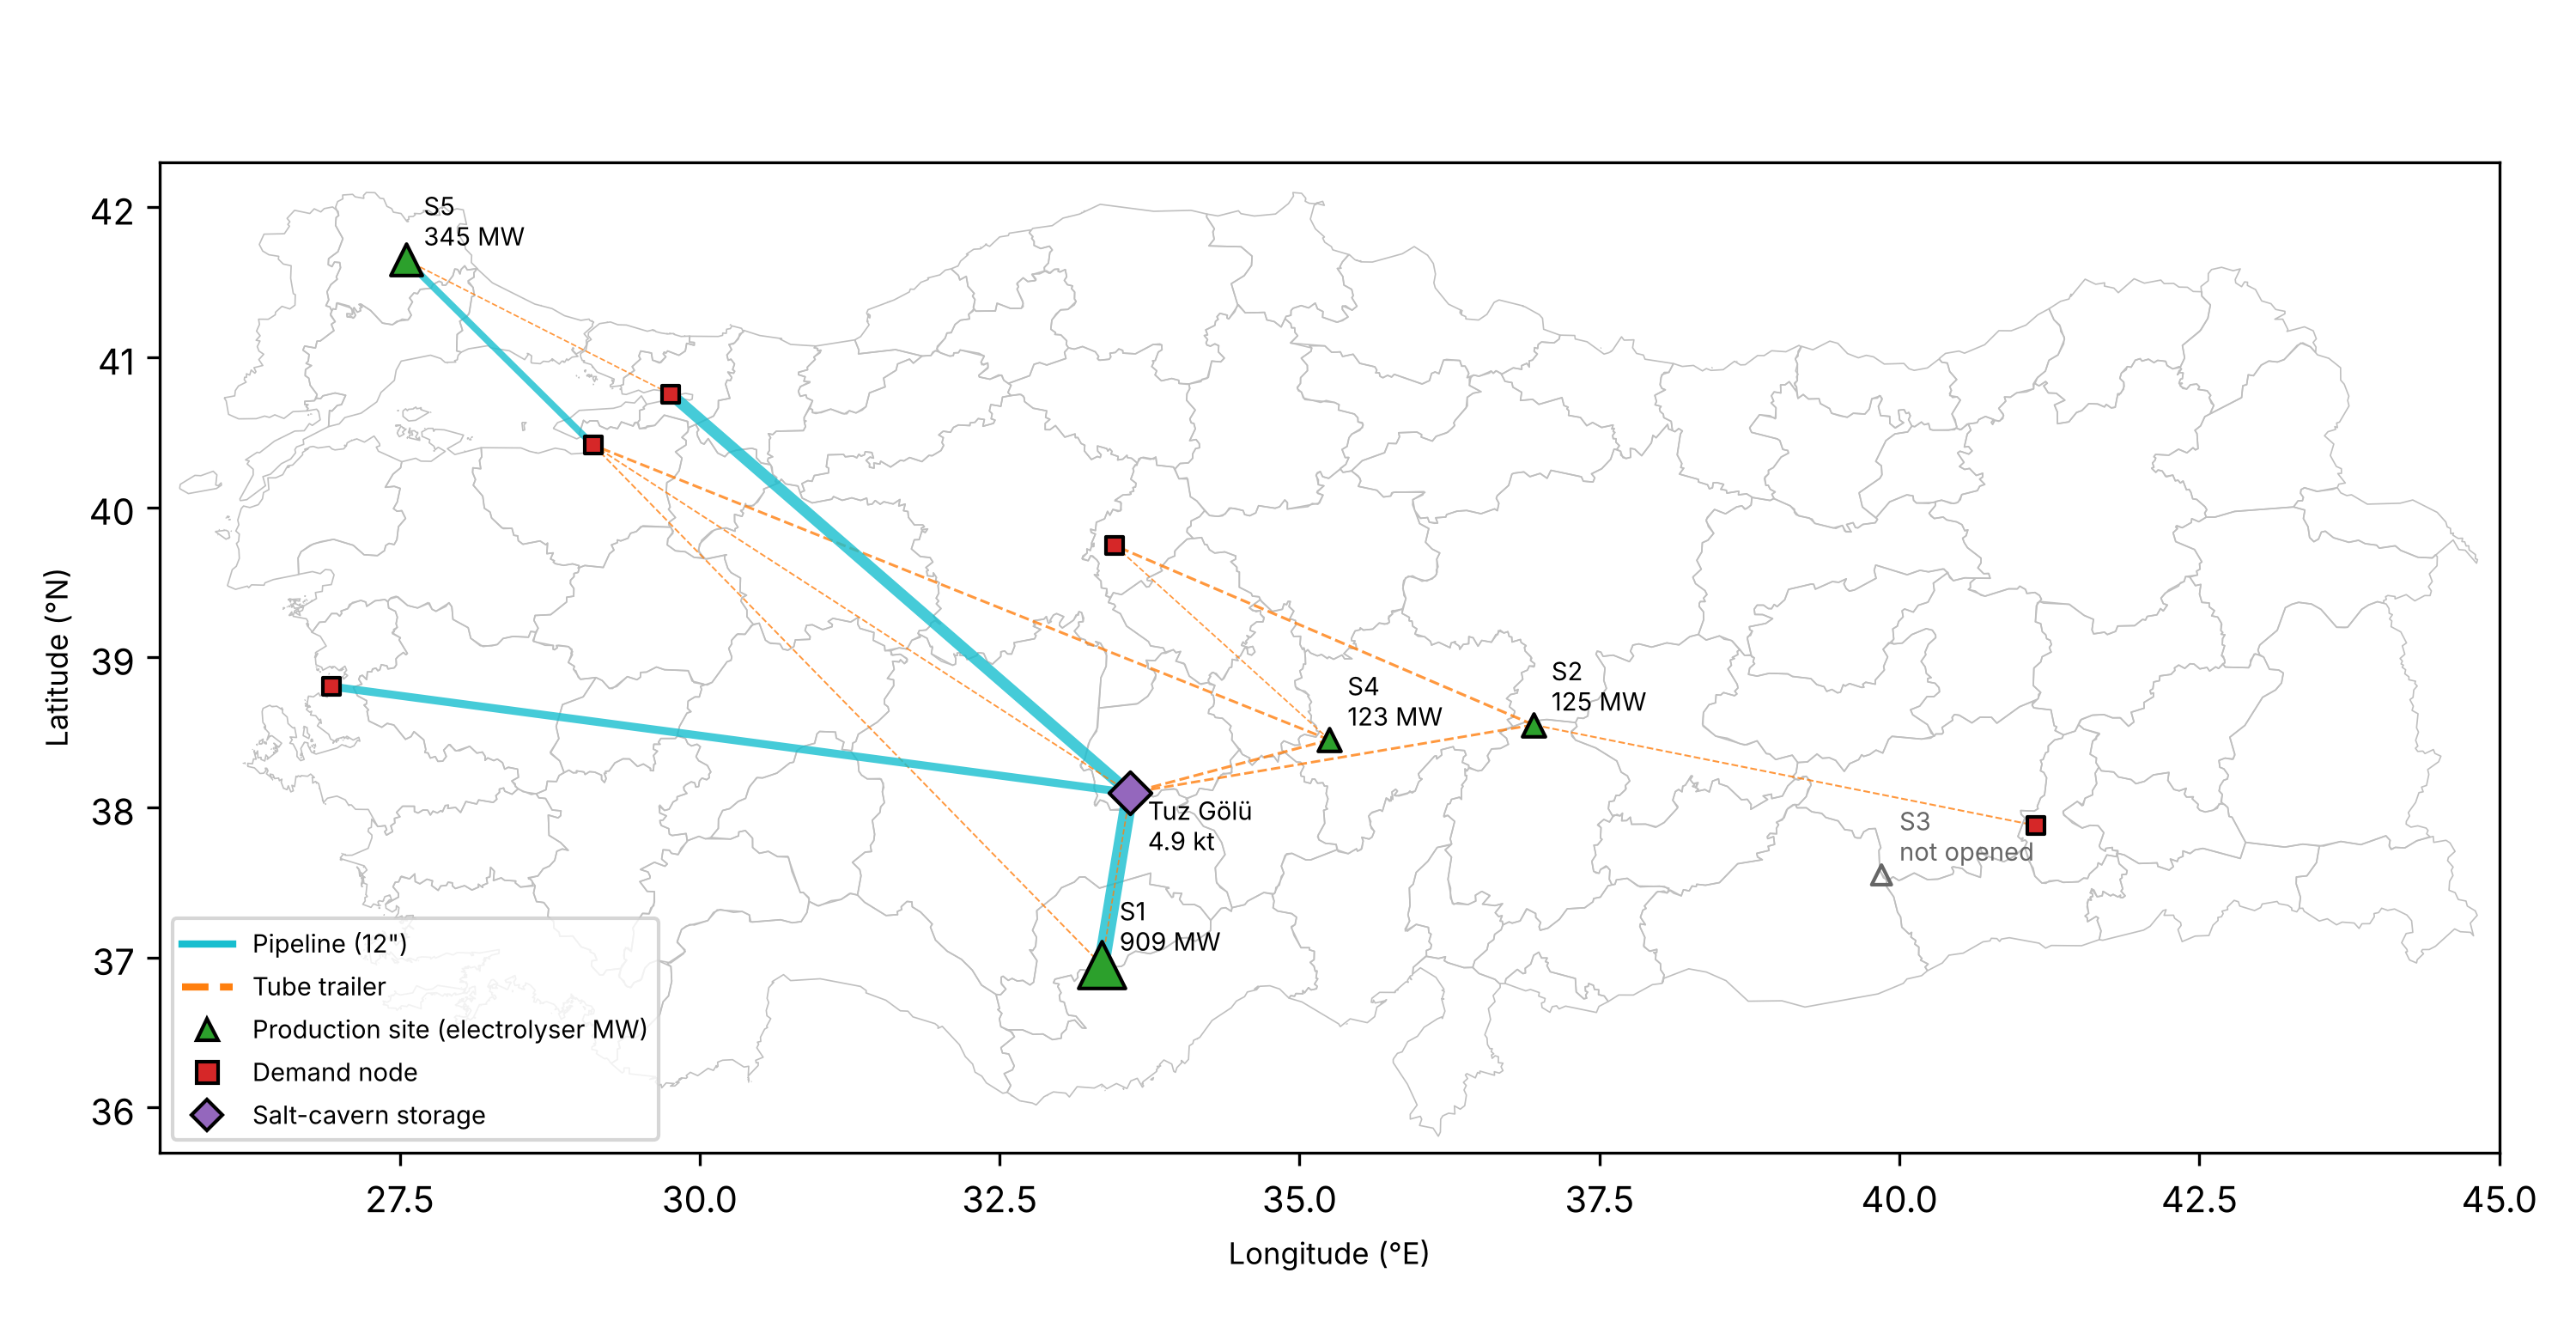
\includegraphics[width=\textwidth]{Fig3_network_base.png}
\caption{Baseline network. Line width is proportional to the annual hydrogen flow; marker size to the electrolyser capacity. Dark blue: 20-inch pipeline; light blue: 12-inch pipeline; dashed: tube trailer.}
\label{fig:network}
\end{figure}

\textit{Network and storage.} Four 12-inch pipelines are built: Karaman (S1) to Tuz Gölü (162\,km), and onward from Tuz Gölü to the Körfez hub (642\,km) and the Aliağa hub (699\,km), together with Kırklareli (S5) to the Gemlik ammonia plant (304\,km). Pipelines make 86\% of final deliveries. Lower wind--PV co-use and annual grid matching reconfigure the corridor altogether (Sections~\ref{sec:stage3_sens} and~\ref{sec:rfnbo}). Trailers make the remaining 14\%, to Kırıkkale, Batman and Gemlik, and also feed the cavern from S2 and S4; Gemlik takes both modes because land binds at Kırklareli, so its pipeline carries the whole of S5's output and the balance of the node's demand arrives by trailer; across all trailer legs the mean haul is 463\,km, the longest 789\,km and the total trailer movement 25.0\,kt/yr, which exceeds the trailer share of final deliveries because the legs feeding the cavern are counted in addition. Tuz Gölü therefore acts as the hub of a corridor towards Marmara and the Aegean: 59.2 of the 60.3\,kt/yr produced at Karaman reach it by pipeline, and 69.4\,kt/yr leave it, 68.5\,kt/yr of them by pipeline. As a seasonal buffer it holds 4.9\,kt of working gas, 8\% of the 62,013\,t potential of the twelve existing caverns, so working-gas volume does not bind at modal demand.

\textit{Cost structure.} Of the 9.96\,€/kg, production accounts for 6.83\,€/kg: electrolysers 3.11, PV 2.76, wind 1.19, stack replacement 0.56 and water 0.03\,€/kg, less export revenue of 0.82\,€/kg. Logistics account for 3.14\,€/kg, of which pipelines make up 71\% (2.23\,€/kg), trailers 0.59\,€/kg, compression 0.16\,€/kg, cavern storage 0.11\,€/kg and grid electricity for injection, refilling and recompression 0.05\,€/kg. Published Turkish estimates are mostly plant-gate costs, comparable with the production component rather than the delivered cost; Supplementary Note~S10 benchmarks the baseline against them.

The modal-value (deterministic) design is the same design, valued at modal parameters at 8.75\,€/kg (Section~\ref{sec:robustness}). The difference between the two costs is a valuation effect, not a design effect: the right skew of several parameters, including proton-exchange membrane (PEM) CAPEX (Supplementary Table~S2), raises the Me expected value above the mode. The range of the baseline cost, from $z_{\min} = 469$ to $z_{\max} = 1{,}882$\,M€/yr, shows how wide this epistemic uncertainty is.

\textit{What changed the logistics result.} A reference configuration of this model --- a single renewable share for all facilities, separate nodes for co-located plants, one pipeline diameter and no long-haul or cavern-refill terms --- delivered 157.9\,kt/yr at 10.70\,€/kg and moved 85\% of the hydrogen by trailer. Table~\ref{tab:ablation} adds the four changes one at a time: the sector-specific demand basis shrinks the network but leaves it trailer-based; shared delivery points and the 12-inch class make pipelines worthwhile at the 20--60\,kt/yr flows the network actually carries; and correcting long-haul trailer costs and costing cavern-side refilling remove the remaining long trailer legs. Trailer dominance was therefore a consequence of the network representation, not of Turkish geography, though how far pipelines displace trailers depends on the pipeline cost level (Section~\ref{sec:stage3_sens}).

\begin{table}[htbp]
\centering
\caption{Stepwise decomposition from a reference configuration to the baseline design. Each row adds one change to the row above. Delivered cost is $E_{\text{Me}}[z]$ per kg delivered.}
\label{tab:ablation}
\resizebox{\textwidth}{!}{%
\begin{tabular}{lrrrrrrl}
\toprule
Configuration & Delivered & Delivered cost & Logistics & of which trailers & Final deliveries & Trailer haul, & Pipelines \\
 & (kt/yr) & (€/kg) & (€/kg) & (€/kg) & share by trailer & mean / max (km) & \\
\midrule
Reference configuration & 157.9 & 10.70 & 3.60 & 2.71 & 0.85 & 694 / 1,421 & 2 $\times$ 20$''$ \\
+ sector-specific demand & 105.2 & 10.26 & 3.54 & 2.93 & 1.00 & 629 / 967 & 1 $\times$ 20$''$ \\
+ shared delivery points & 105.2 & 10.19 & 3.47 & 1.79 & 0.60 & 639 / 1,064 & 2 $\times$ 20$''$ \\
+ 12-inch class & 105.2 & 9.77 & 2.97 & 1.30 & 0.39 & 727 / 1,064 & 3 $\times$ 12$''$ \\
+ long-haul and refill costs (baseline) & 105.2 & 9.96 & 3.14 & 0.59 & 0.14 & 463 / 789 & 4 $\times$ 12$''$ \\
\bottomrule
\end{tabular}%
}
\end{table}

\subsection{Sensitivity of the Network Design}
\label{sec:stage3_sens}
Table~\ref{tab:stage3_scenarios} reports the single-objective sensitivity runs. Four patterns stand out.
\begin{enumerate}
    \item \textit{Land basis.} Cluster-level land, the second baseline, lowers the delivered cost by 13\% to 8.64\,€/kg and concentrates production at Karaman and Kırklareli, which then have room for 2.0\,GW of wind. Lower wind--PV co-use raises cost (10.22\,€/kg at $\phi=0.5$, 10.62\,€/kg at $\phi=0$) and shifts the pipeline layout from a Tuz Gölü hub to direct lines from Karaman to Aliağa and from Kayseri to Körfez.
    \item \textit{Logistics assumptions.} Trailer operating hours of 4,400 or 8,000 move the cost by less than 0.1\,€/kg, and capping pipeline length at 1.2 times the geodesic distance lowers it to 9.72\,€/kg, a lower-bound illustration rather than a routed design. Raising the 12-inch capacity to the value implied by velocity-limited sizing \citep{dea2025hydrogen} leaves the network unchanged. The pipeline cost level matters more for the layout than for the cost: under the Danish Energy Agency datasheet values \citep{dea2025datasheet} the Aliağa line is replaced by trailers (10.09\,€/kg, trailer share 39\%), and adding that datasheet's 35\% construction-management and owner's costs to both diameters also removes the Kırklareli--Gemlik line (10.45\,€/kg, 60\%). The Karaman--Tuz Gölü--Körfez spine is built in all three cases.
    \item \textit{Electricity and efficiency.} Without surplus sales the cost rises to 10.53\,€/kg; annual-matched grid imports are discussed in Section~\ref{sec:rfnbo}. The electrolyser's electricity consumption moves the cost between 8.95 ($\eta=48$\,kWh/kg) and 10.35\,€/kg ($\eta=57.5$\,kWh/kg).
    \item \textit{Decision attitude and scale.} Varying $\lambda$ changes the valuation (8.30--11.63\,€/kg) far more than the design, and $\gamma$ barely changes either over its admissible range $0\le\gamma\le(1-\lambda)/2$. The upper-bound demand basis (157.9\,kt/yr) opens all five sites and lowers the cost per kilogram to 9.60\,€/kg through scale.
\end{enumerate}
In every run the modal demand is met and the 12-inch class carries all pipeline flow.

\begin{table}[htbp]
\centering
\caption{Stage~III sensitivity runs (single objective). Delivered cost is $E_{\text{Me}}[z]$ per kg delivered (modal values for the deterministic run); $\bar{\alpha}$ is the mean confidence level over the demand nodes; the trailer column is the share of final deliveries made by trailer. The $\delta$ runs apply a uniform import parity to all facilities.}
\label{tab:stage3_scenarios}
\resizebox{\textwidth}{!}{%
\begin{tabular}{lrrrrrrrllrr}
\toprule
Run & Delivered cost & Delivered & $\bar{\alpha}$ & Wind & PV & Electrolyser & Cavern & Open sites & Pipelines & Trailer & $\bar{Q}$ \\
 & (€/kg) & (kt/yr) & & (GW) & (GW) & (GW) & (kt) & & & share & \\
\midrule
%<<GEN:tab_sensitivity>>
Baseline (cell land, $\phi=1$) & 9.96 & 105.2 & 0.50 & 0.82 & 3.31 & 1.50 & 4.9 & S1, S2, S4, S5 & 4$\times$12$^{\prime\prime}$ & 0.14 & 0.523 \\
Deterministic (modal values, $\gamma = 0$) & 8.75 & 105.2 & 0.50 & 0.82 & 3.36 & 1.51 & 4.6 & S1, S2, S4, S5 & 4$\times$12$^{\prime\prime}$ & 0.14 & 0.523 \\
Cluster-level land (second baseline) & 8.64 & 105.2 & 0.50 & 1.99 & 1.65 & 1.07 & 2.9 & S1, S5 & 3$\times$12$^{\prime\prime}$ & 0.36 & 0.528 \\
Co-use $\phi=0.5$ & 10.22 & 105.2 & 0.50 & 0.76 & 3.25 & 1.53 & 4.6 & S1, S2, S4, S5 & 2$\times$12$^{\prime\prime}$ & 0.38 & 0.524 \\
Exclusive land $\phi=0$ & 10.62 & 105.2 & 0.50 & 0.63 & 3.48 & 1.62 & 4.8 & S1, S2, S3, S4, S5 & 3$\times$12$^{\prime\prime}$ & 0.35 & 0.522 \\
S-island (no surplus sales) & 10.53 & 105.2 & 0.50 & 0.65 & 3.03 & 1.68 & 4.6 & S1, S2, S4, S5 & 4$\times$12$^{\prime\prime}$ & 0.13 & 0.523 \\
S-grid (annual matching) & 8.07 & 105.2 & 0.50 & 0.66 & 2.75 & 1.08 & 0.0 & S1, S3, S4, S5 & 3$\times$12$^{\prime\prime}$ & 0.07 & 0.549 \\
$\eta = 48$\,kWh/kg & 8.95 & 105.2 & 0.50 & 0.59 & 3.10 & 1.35 & 4.3 & S1, S4, S5 & 4$\times$12$^{\prime\prime}$ & 0.13 & 0.522 \\
$\eta = 57.5$\,kWh/kg & 10.35 & 105.2 & 0.50 & 0.82 & 3.43 & 1.59 & 4.9 & S1, S2, S4, S5 & 4$\times$12$^{\prime\prime}$ & 0.15 & 0.523 \\
Trailer hours 4,400\,h/yr & 10.02 & 105.2 & 0.50 & 0.79 & 3.32 & 1.52 & 4.8 & S1, S2, S4, S5 & 4$\times$12$^{\prime\prime}$ & 0.14 & 0.522 \\
Trailer hours 8,000\,h/yr & 9.94 & 105.2 & 0.50 & 0.82 & 3.31 & 1.50 & 4.9 & S1, S2, S4, S5 & 4$\times$12$^{\prime\prime}$ & 0.14 & 0.522 \\
Pipeline length $\le 1.2\times$ geodesic & 9.72 & 105.2 & 0.50 & 0.82 & 3.30 & 1.50 & 4.9 & S1, S2, S4, S5 & 4$\times$12$^{\prime\prime}$ & 0.13 & 0.522 \\
12-inch capacity 311\,t/d & 9.96 & 105.2 & 0.50 & 0.82 & 3.30 & 1.51 & 4.9 & S1, S2, S4, S5 & 4$\times$12$^{\prime\prime}$ & 0.14 & 0.522 \\
12-inch cost and capacity, DEA (2025) & 10.09 & 105.2 & 0.50 & 0.82 & 3.36 & 1.49 & 4.9 & S1, S2, S4, S5 & 3$\times$12$^{\prime\prime}$ & 0.39 & 0.523 \\
Pipeline CAPEX $+35\%$ (DEA owner's costs) & 10.45 & 105.2 & 0.50 & 0.82 & 3.36 & 1.48 & 4.7 & S1, S2, S4, S5 & 2$\times$12$^{\prime\prime}$ & 0.60 & 0.521 \\
Upper-bound demand (42\% for all) & 9.60 & 157.9 & 0.50 & 0.92 & 4.96 & 2.49 & 7.7 & S1, S2, S3, S4, S5 & 5$\times$12$^{\prime\prime}$ & 0.14 & 0.523 \\
$\gamma = 0$ & 9.96 & 105.2 & 0.50 & 0.82 & 3.39 & 1.49 & 4.9 & S1, S2, S4, S5 & 4$\times$12$^{\prime\prime}$ & 0.14 & 0.523 \\
$\gamma = 0.25$ & 9.97 & 105.2 & 0.50 & 0.82 & 3.30 & 1.51 & 4.9 & S1, S2, S4, S5 & 4$\times$12$^{\prime\prime}$ & 0.14 & 0.522 \\
$\lambda = 0.25$ & 8.30 & 105.2 & 0.25 & 0.82 & 3.34 & 1.50 & 4.9 & S1, S2, S4, S5 & 4$\times$12$^{\prime\prime}$ & 0.14 & 0.523 \\
$\lambda = 0.75$ & 11.63 & 105.2 & 0.75 & 0.80 & 3.30 & 1.51 & 4.9 & S1, S2, S4, S5 & 4$\times$12$^{\prime\prime}$ & 0.14 & 0.522 \\
$\delta = 10$ & 9.96 & 105.2 & 0.50 & 0.82 & 3.31 & 1.50 & 4.9 & S1, S2, S4, S5 & 4$\times$12$^{\prime\prime}$ & 0.14 & 0.523 \\
$\delta = 12.5$ & 9.57 & 156.0 & 0.79 & 0.92 & 4.94 & 2.44 & 7.5 & S1, S2, S3, S4, S5 & 5$\times$12$^{\prime\prime}$ & 0.10 & 0.523 \\
$\delta = 15$ & 9.63 & 164.7 & 0.90 & 0.92 & 5.13 & 2.66 & 8.0 & S1, S2, S3, S4, S5 & 5$\times$12$^{\prime\prime}$ & 0.13 & 0.523 \\
$\delta = 20$ & 9.86 & 177.0 & 1.00 & 1.09 & 6.26 & 2.62 & 9.7 & S1, S2, S3, S4, S5 & 5$\times$12$^{\prime\prime}$ & 0.14 & 0.519 \\
%<<END>>
\bottomrule
\end{tabular}%
}
\end{table}

\subsection{What the Ranking and the Robust Formulation Change}
\label{sec:robustness}
\textit{The ranking.} Table~\ref{tab:counterfactual} compares the integrated design with a sequential one in which the ranking is used as a pre-filter: only the three highest-ranked candidates (S5, S4, S2) are admitted, and the network is then optimised for cost. Excluding Karaman, the lowest-ranked but largest and cheapest site, raises the delivered cost by 11\%, from 9.96 to 11.07\,€/kg under the RPP valuation and from 8.75 to 9.72\,€/kg at modal values, and the Monte Carlo mean cost by 120\,M€/yr. In exchange, $\bar Q$ rises from 0.523 to 0.536, almost the maximum attainable (0.537). The sequential design thus lands at the expensive end of the integrated Pareto front (Section~\ref{sec:pareto}), whereas the knee of that front captures 60\% of the same suitability gain for 22\% of the cost increase. The cost-minimising end of an $\varepsilon$-constraint front is by construction the cost-only optimum, so the informative test is the sequential counterfactual rather than the end point itself: the value of coupling the ranking to the network lies in pricing the preference.

\begin{table}[htbp]
\centering
\caption{Integrated and sequential designs. Delivered cost is $E_{\text{Me}}[z]$ per kg delivered (modal values for the deterministic designs); $f_1$ is the robust objective in M€/yr.}
\label{tab:counterfactual}
\resizebox{\textwidth}{!}{%
\begin{tabular}{lrrrll}
\toprule
Design & Delivered cost (€/kg) & $f_1$ (M€/yr) & $\bar Q$ & Open sites & Pipelines \\
\midrule
%<<GEN:tab_counterfactual>>
Integrated RPP (all candidates, suitability objective at cost optimum) & 9.96 & 1,813 & 0.523 & S1, S2, S4, S5 & 4$\times$12$^{\prime\prime}$ \\
Deterministic (all candidates) & 8.75 & 921 & 0.523 & S1, S2, S4, S5 & 4$\times$12$^{\prime\prime}$ \\
Sequential: top-3 by ranking, then RPP & 11.07 & 1,947 & 0.536 & S2, S4, S5 & 4$\times$12$^{\prime\prime}$ \\
Sequential: top-3 by ranking, then deterministic & 9.72 & 1,022 & 0.536 & S2, S4, S5 & 4$\times$12$^{\prime\prime}$ \\
%<<END>>
\bottomrule
\end{tabular}%
}
\end{table}

\textit{The robust formulation.} At the baseline import parity every confidence level stays at its lower bound ($\alpha_j=\lambda$), and the RPP design has the same sites and pipelines as the deterministic design and nearly the same capacities. Written out, the RPP objective at $\lambda=0.5$ and $\gamma=0.2$ is a deterministic MILP with pessimistically shifted coefficients plus a penalty on the possible demand violation, so a different design arises only if the shifted coefficients change the ranking of options or the penalty makes hedging worthwhile. Neither happens at the baseline: the two designs have practically indistinguishable Monte Carlo cost distributions (Table~\ref{tab:mc}). The design is unchanged up to $\delta=10$\,€/kg; hedging begins between 10 and 12.5\,€/kg and reaches the full possibility range at $\delta=20$\,€/kg, where all five sites open (Table~\ref{tab:stage3_scenarios}). Because hedged capacity runs at higher output, the delivered cost per kilogram falls slightly while total cost rises.

Across 10,000 joint draws, the system-wide shortfall probability of the modal designs is 0.77, and at least one node is short in 84\% of draws. Hedging raises mean cost; it pays off on average only if unmet demand costs 32\,€/kg ($\delta = 12.5$ design), 35\,€/kg ($\delta=15$) or 39\,€/kg ($\delta=20$). Below these prices the moderately hedged designs ($\delta=12.5$ and $\delta=15$) are insurance: they lower the 95th percentile once unmet demand costs about 20\,€/kg or more; the fully hedged $\delta=20$ design does so only above about 30\,€/kg. At $\delta = 20$\,€/kg the RPP design secures the whole possibility range, so decision makers with probabilistic demand beliefs may prefer a lower penalty.

\textit{Imports.} The demand constraint makes domestic supply of the modal demand mandatory. Lifting it, so that imports at parity may replace any part of the demand, makes the model import everything at 5.63, 7.30 and a uniform 10\,€/kg; at 12.5\,€/kg it produces 89\,kt/yr domestically. The domestic network therefore competes with imports only above roughly 10--12.5\,€/kg and otherwise rests on the security-of-supply mandate.

\textit{Monte Carlo reading.} The Monte Carlo samples the same annualised coefficient triangles as the RPP; Supplementary Note~S11 reconciles its mean with the Me expected value.

\begin{table}[htbp]
\centering
\caption{Monte Carlo evaluation of fixed designs ($N = 10{,}000$; common random numbers; coefficients sampled from the RPP's annualised triangles). Total cost adds unmet demand valued at the uniform import price shown. P(shortfall) is the system-level probability that total demand exceeds total delivery.}
\label{tab:mc}
\resizebox{\textwidth}{!}{%
\begin{tabular}{lrrrrrrr}
\toprule
Design & Cost mean & Cost P95 & P(shortfall) & Mean shortfall & \multicolumn{3}{c}{Total cost mean / P95 (M€/yr) at import price} \\
\cmidrule(lr){6-8}
 & (M€/yr) & (M€/yr) & & (kt/yr) & 7.30\,€/kg & 20\,€/kg & 30\,€/kg \\
\midrule
%<<GEN:tab_mc>>
Deterministic & 1,093 & 1,336 & 0.77 & 18.9 & 1,231 / 1,570 & 1,471 / 2,202 & 1,660 / 2,735 \\
Baseline RPP & 1,093 & 1,334 & 0.77 & 18.9 & 1,230 / 1,568 & 1,470 / 2,202 & 1,659 / 2,734 \\
RPP, $\delta = 12.5$ & 1,559 & 1,930 & 0.07 & 4.5 & 1,592 / 1,970 & 1,649 / 2,055 & 1,694 / 2,136 \\
RPP, $\delta = 15$ & 1,656 & 2,055 & 0.02 & 2.9 & 1,676 / 2,080 & 1,713 / 2,130 & 1,741 / 2,174 \\
RPP, $\delta = 20$ & 1,820 & 2,244 & 0.00 & 0.0 & 1,820 / 2,244 & 1,820 / 2,244 & 1,820 / 2,244 \\
Sequential top-3 (deterministic) & 1,213 & 1,492 & 0.77 & 18.9 & 1,350 / 1,714 & 1,590 / 2,336 & 1,779 / 2,857 \\
Co-use $\phi = 0.5$ & 1,120 & 1,362 & 0.77 & 18.9 & 1,258 / 1,599 & 1,498 / 2,229 & 1,687 / 2,763 \\
Exclusive land $\phi = 0$ & 1,163 & 1,415 & 0.77 & 18.9 & 1,301 / 1,649 & 1,541 / 2,278 & 1,730 / 2,808 \\
%<<END>>
\bottomrule
\end{tabular}%
}
\end{table}

\subsection{Cost--Suitability Pareto Front}
\label{sec:pareto}
Figure~\ref{fig:pareto} shows seven Pareto solutions, each within a 0.1\% MIP gap; the augmentation term of AUGMECON2 is scaled by the range of the second objective, so that it is of the same order as the solver tolerance. Under the baseline land basis and renewable-only supply, production-weighted suitability can rise only from 0.523 to 0.537, because the candidate scores are close and Kırklareli, the highest-ranked site, is land-constrained.

The knee lies at $\bar{Q} = 0.531$. Up to the knee, $\bar Q$ rises by 0.008 while the robust objective $f_1$ rises by 1.5\% and the delivered cost $E_{\text{Me}}[z]$ from 9.96 to 10.21\,€/kg; S1's output falls from 60.3 to 25.5\,kt/yr and S4's rises from 10.9 to 42.3\,kt/yr. Beyond the knee, the last 0.006 of $\bar Q$ costs a further 6.0\% of $f_1$ and raises the delivered cost to 11.09\,€/kg, as S1 is closed and S3 opened. Changes are reported in absolute $\bar Q$, since $Q^{01}$ is an interval-scale score whose percentage changes depend on its affine rescaling.

\begin{figure}[htbp]
\centering
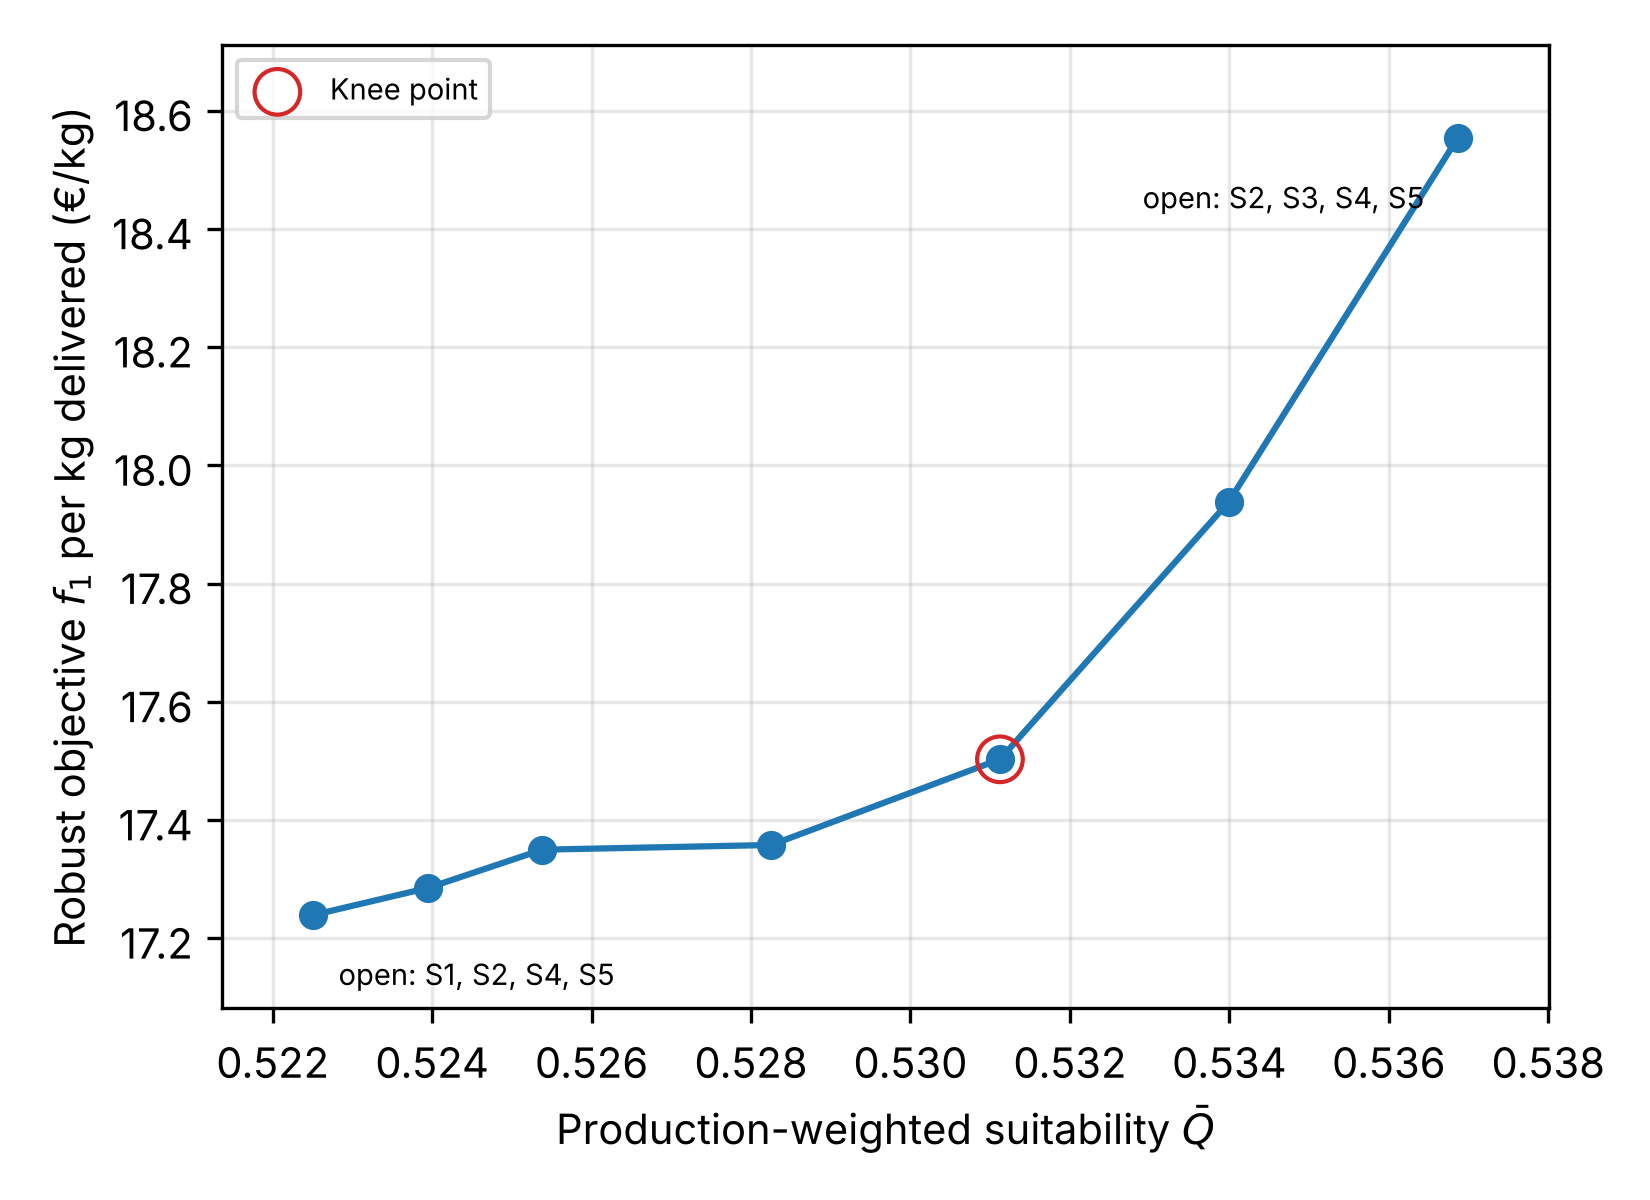
\includegraphics[width=0.7\textwidth]{Fig4_pareto_base.png}
\caption{Pareto front between the robust possibilistic objective $f_1$, here divided by the annual delivery to give €/kg (it exceeds $E_{\text{Me}}[z]$ by the range and violation penalties), and the production-weighted suitability $\bar{Q}$ (AUGMECON2; hybrid spherical-fuzzy CRITIC--WASPAS scores $Q_i$). The circle marks the knee point.}
\label{fig:pareto}
\end{figure}

\subsection{Electricity Sourcing and RFNBO Compliance}
\label{sec:rfnbo}
Because electrolysis uses only co-located new renewable electricity, the emissions that count against the RFNBO threshold of 3.38\,kgCO$_2$e/kg are those of logistics: diesel for tube trailers, at 32.6\,L/100\,km for a typical EU tractor-trailer \citep{icct2018fuel} and 3.12\,kgCO$_2$e/L well-to-wheel \citep{desnz2024ghg} including empty return trips, and grid electricity for cavern injection, trailer refilling at the cavern and pipeline recompression at 0.436\,tCO$_2$e/MWh.

With 1,000\,kg trailers the baseline emits 0.56\,kgCO$_2$e/kg on average: 0.33 from grid electricity, mostly for cavern injection and refilling, and 0.22 from trailers. It complies comfortably, as do all renewable-only runs and all Pareto points; the highest renewable-only value, 0.86\,kgCO$_2$e/kg, occurs under cluster-scale land. Because pipelines carry most of the hydrogen, compliance no longer hinges on the trailer technology: with 300\,kg trailers (Type~I steel tubes) the baseline average rises to 1.08\,kgCO$_2$e/kg, against 4.16\,kgCO$_2$e/kg in the trailer-based reference configuration. Single legs remain a risk if compliance is assessed per delivery: the longest trailer leg (789\,km) emits 1.6\,kgCO$_2$e/kg with 1,000\,kg trailers and 5.4\,kgCO$_2$e/kg with 300\,kg trailers.

Annual matching through YEK-G certificates lowers the delivered cost by 1.90\,€/kg (to 8.07\,€/kg), while total grid electricity raises the calculated carbon intensity to 11.3\,kgCO$_2$e/kg, 3.3 times the RFNBO threshold and equal to the fossil comparator (94\,gCO$_2$e/MJ). The S-grid design draws 2.71\,TWh/yr of grid electricity in total, including that used for pipeline recompression; the matching constraint compares only weighted site-level imports with exports. Hydrogen produced this way would not qualify as renewable under EU rules, so the cost advantage of annual matching is the value of that lost qualification. Grid dependency is pivotal in both directions: \citet{devrim2026comprehensive} find that grid imports raise the levelised cost of a fixed hybrid plant, because they cover a capacity shortfall there, whereas here they substitute for dedicated capacity and lower it.

\subsection{Policy Implications}
Five implications follow, each tied to the runs that support it.
\begin{enumerate}
    \item \textit{Plan a 12-inch corridor rather than trailer logistics.} Because 12-inch pipelines dominate every run while the optimal routing shifts across scenarios (Tables~\ref{tab:ablation} and~\ref{tab:stage3_scenarios}), corridor planning should fix the 12-inch capacity class, sized for the 20--60\,kt/yr flows the network actually carries rather than for the 20-inch European backbone, while keeping the routing flexible.
    \item \textit{Treat domestic supply as an explicit policy choice.} Since unrestricted imports undercut domestic production up to 10--12.5\,€/kg (Section~\ref{sec:robustness}), instruments such as contracts for difference would have to bridge a gap of several euros per kilogram.
    \item \textit{Size domestic production to the modal demand.} Because hedging the upper demand tail raises expected cost unless shortfall penalties exceed 32\,€/kg (Section~\ref{sec:robustness}), domestic capacity should target the modal demand while import contracts cover the tail.
    \item \textit{Enable cluster-scale development.} Admitting cluster-wide eligible land cuts the delivered cost materially and concentrates output at two sites (Table~\ref{tab:stage3_scenarios}); permitting and private-wire connection rules across tens of kilometres are the corresponding regulatory levers.
    \item \textit{Address water before interior production scales.} The interior candidates supply most of the baseline output but lie in basins with extremely high water-stress scores (Table~\ref{tab:stage2_results}), and basin-level abstraction limits are not modelled (Section~\ref{sec:limits}), so water allocation should be assessed when permitting interior projects rather than assumed.
\end{enumerate}
If export to the EU is an objective, hourly matching and low-emission logistics must be built into project design from the outset, because annual matching yields cheaper but non-compliant hydrogen (Section~\ref{sec:rfnbo}).

\section{Conclusion}
This study asked whether expert-informed siting preferences and possibilistic hedging change a national green hydrogen network when land and logistics constrain it. It combined pixel-level GIS screening, a hybrid spherical-fuzzy CRITIC--WASPAS ranking, a seasonal robust possibilistic network model and a Monte Carlo evaluation on the same coefficients, and tested each layer against a counterfactual.

Serving the modal 2030 renewable demand of 105.2\,kt/yr costs 9.96\,€/kg delivered, and 12-inch pipelines towards Marmara and the Aegean, not trailer haulage, carry most of the hydrogen; the Karaman--Tuz Gölü--Körfez spine holds under every pipeline cost estimate tested. The siting ranking does not change the cost-optimal network, and its value is in pricing preference: a pre-filter based on it costs 11\% more than the cost-optimal design. The robust formulation coincides with the deterministic design at import parity, hedging pays only above about 32\,€/kg, and domestic supply competes with imports only above roughly 10--12.5\,€/kg. Renewable-only supply meets the RFNBO threshold at system level even with low-capacity trailers, although individual long trailer legs do not, whereas annual grid matching fails outright. These findings are conditional on the expert panel, the demand benchmark and single-year weather data.

\subsection{Limitations and Future Research}
\label{sec:limits}
The results are subject to the following limitations.
\begin{itemize}
    \item \textit{Expert judgement.} Three of the seven Stage~II criteria (K5--K7) and the subjective component of the weights come from a panel of four experts. The ranking is stable under weight perturbation, leave-one-criterion-out, leave-one-expert-out and six method variants, but none addresses whether four respondents represent the relevant professional community. Because $Q^{01}$ enters the second Stage~III objective, the cost--suitability front is conditional on the panel.
    \item \textit{Demand basis.} The refinery share applies the RED III transport sub-target as if it were met entirely through refinery hydrogen, which bounds the refinery role from above; Türkiye is not bound by RED III, and the modal demand is a benchmark for export-oriented producers rather than a forecast. The upper-bound scenario (157.9\,kt/yr) brackets the alternative reading.
    \item \textit{Data and parameters.} Hourly profiles use the single year 2023, and the ERA5 wind speeds were scaled to the Global Wind Atlas capacity factors by factors of up to 2.04, which preserves the hourly shape but leaves its local accuracy uncertain. Technical coefficients are held at modal values and varied only in scenarios. Most cost parameters are European or United States (US) values, several from secondary compilations; the 12-inch pipeline class is extrapolated below the smallest European Hydrogen Backbone class, with a modal cost the Danish Energy Agency datasheet confirms over a narrower range; the Tuz Gölü injection and withdrawal rates are scaled from natural-gas design rates. Supplementary Table~S2 records the source and evidence level of every parameter.
    \item \textit{Water.} Raw-water use is parameterised at 17.5\,L/kg (range 8.9--26.5), about 1.8 million\,m$^3$/yr for the baseline network. Basin-level abstraction limits are not modelled, because no verified open spatial dataset was available for the candidate basins, so water stress enters only through the Stage~II ranking.
    \item \textit{Imports and the domestic-supply mandate.} The modal demand is supplied domestically by construction (Section~\ref{sec:stage3_base}); the import diagnostic shows that this is a policy choice rather than a cost-optimal outcome. Import parities are single crisp values based on European delivery points.
    \item \textit{Storage and emissions.} Seasonal storage is linked across season boundaries only, so day-to-day inventory within a season is not tracked and the working-gas requirement may be understated; the model covers a single investment year (2030); and emissions are evaluated at system and leg level rather than per consignment. Purification after cavern withdrawal is not costed, although water uptake from the brine makes a drying step likely \citep{janssen2025assessment}. Storage is restricted to salt caverns, which suits the Turkish case because Tuz Gölü is the only developed prospect.
    \item \textit{Candidate set.} Stage~I fixes five candidates through its clustering and spacing rules; the framework offers one way of generating them and does not claim that five is optimal. A different selection rule, spacing threshold or number of candidates would change the Stage~II alternatives and, through them, the Stage~III design, so the results are conditional on the screening parameters reported in Supplementary Table~S8.
    \item \textit{Logistics and routing.} Trailer transport is represented by levelised costs with a trip-feasibility correction rather than an explicit fleet schedule, and intra-day balancing is assumed to come from line pack and on-site trailers. Arc lengths are OSRM road distances used as a proxy for pipeline corridors, and the network allows point-to-point lines and shared delivery points but no general branching.
    \item \textit{Asset outages and uncertainty.} Full-year outages of the cavern and of the most heavily used pipeline are tested with the investment re-optimised for maximum delivery, which raises the delivered cost to 10.81 and 10.05\,€/kg respectively (Supplementary Table~S6); partial and 30-day outages are not represented by the seasonal time structure. The Monte Carlo evaluation reads the possibility distributions as independent triangular probability distributions, keeps each design fixed without re-dispatch, and does not sample weather or technical coefficients.
\end{itemize}

Future work should extend the model to 2030--2040 steel demand and electrolyser learning, represent trailer fleets and consignment-level emissions, add basin-level water constraints, optimise the routing of the corridor with branching pipelines, add multi-year weather and re-dispatch to the Monte Carlo evaluation, and broaden expert elicitation through Delphi.

\section*{CRediT authorship contribution statement}
\textbf{Kadir Sarıkaya:} Conceptualization, Methodology, Software, Validation, Formal analysis, Investigation, Data curation, Writing --- original draft, Writing --- review \& editing, Visualization, Project administration.

\section*{Declaration of Competing Interests}
The author declares no competing interests.

\section*{Funding}
This research did not receive any specific grant from funding agencies in the public, commercial, or not-for-profit sectors.

\section*{Ethical approval and consent to participate}
Not applicable. The study does not involve human participants, animal experiments, or confidential data.

\section*{Data Availability}
The parameter set, code, frozen open-data inputs, processed aggregate results, the supplementary tables as machine-readable CSV files, and the reproduction checks are available at \texttt{https://github.com/k-sarikaya/GIS-Hydrogen}. 

\section*{Declaration of generative AI and AI-assisted technologies in the manuscript preparation process}
During the preparation of this work, the author used generative AI technologies to assist with manuscript consistency checks and language editing. After using these tools, the author reviewed and edited and takes full responsibility for the content of the manuscript.

\bibliographystyle{elsarticle-harv}
\begin{thebibliography}{99}
\bibitem[AIIB(2018)]{aiib2018tuzgolu}
Asian Infrastructure Investment Bank (AIIB), 2018. Project Document: Republic of Turkey -- Turkey Gas Storage Expansion Project (Project No.~000062). AIIB, Beijing. https://www.aiib.org/en/projects/approved/2018/\_download/turkey/document/turkey-gas-storage-expansion.pdf

\bibitem[Ajanovic et~al.(2024)]{ajanovic2024future}
Ajanovic, A., Sayer, M., Haas, R., 2024. On the future relevance of green hydrogen in Europe. Applied Energy 358, 122586. https://doi.org/10.1016/j.apenergy.2023.122586

\bibitem[Ali et~al.(2026)]{ali2026optimal}
Ali, T., Aytekin, A., Demidionov, M., 2026. Optimal siting of wind powered green hydrogen production in Bangladesh using interval-valued T-spherical fuzzy multi-criteria decision-making method. International Journal of Hydrogen Energy 217, 153931. https://doi.org/10.1016/j.ijhydene.2026.153931

\bibitem[Atanassov(1986)]{atanassov1986intuitionistic}
Atanassov, K.T., 1986. Intuitionistic fuzzy sets. Fuzzy Sets and Systems 20~(1), 87--96. https://doi.org/10.1016/S0165-0114(86)80034-3

\bibitem[Bairamzadeh et~al.(2016)]{bairamzadeh2016multi}
Bairamzadeh, S., Pishvaee, M.S., Saidi-Mehrabad, M., 2016. Multiobjective robust possibilistic programming approach to sustainable bioethanol supply chain design under multiple uncertainties. Industrial \& Engineering Chemistry Research 55~(1), 237--256. https://doi.org/10.1021/acs.iecr.5b02875

\bibitem[Baki(2022)]{baki2022botas}
Baki, E.S., 2022. BOTA{\c{S}} Hidrojen {\c{C}}al{\i}{\c{s}}malar{\i} [BOTA{\c{S}} hydrogen activities]. Presentation, Towards 2053: The Future of Thermal Power Plants Workshop, 25--26 May 2022, Ministry of Energy and Natural Resources and E{\"U}A{\c{S}}, Ankara (in Turkish).

\bibitem[Becker et~al.(2024)]{becker2023integrated}
Becker, T., Wolff, M., Linzenich, A., Engelmann, L., Arning, K., Ziefle, M., et~al., 2024. An integrated bi-objective optimization model accounting for the social acceptance of renewable fuel production networks. European Journal of Operational Research 315~(1), 354--367. https://doi.org/10.1016/j.ejor.2023.11.044

\bibitem[Bynum et~al.(2021)]{bynum2021pyomo}
Bynum, M.L., Hackebeil, G.A., Hart, W.E., Laird, C.D., Nicholson, B.L., Siirola, J.D., et~al., 2021. Pyomo: Optimization Modeling in Python. 3rd Edition. Springer Optimization and Its Applications, vol.~67. Springer, Cham. https://doi.org/10.1007/978-3-030-68928-5

\bibitem[Camelo et~al.(2025)]{camelo2025milp}
Camelo, M.M., de~Andrade, C.F., de~Athayde Prata, B.A., 2025. A mixed-integer linear programming model for optimizing green hydrogen supply chain networks. International Journal of Hydrogen Energy 118, 134--145. https://doi.org/10.1016/j.ijhydene.2025.02.138

\bibitem[CATF(2025)]{catf2025hydrogen}
Clean Air Task Force (CATF), 2025. Hydrogen in EU Industry: Decarbonising Existing Hydrogen Production and Consumption in the EU 27. Clean Air Task Force, Boston, MA. https://www.catf.us/resource/hydrogen-in-eu-industry/

\bibitem[Çelikdemir and Özdemir(2026)]{celikdemir2026hubs}
Çelikdemir, S., Özdemir, M.T., 2026. Multi-criteria optimization of green hydrogen hubs in T{\"u}rkiye with integration to the Asia-Europe hydrogen corridor. International Journal of Hydrogen Energy 215, 153772. https://doi.org/10.1016/j.ijhydene.2026.153772

\bibitem[Clean Hydrogen Partnership(2026)]{cho2026red}
Clean Hydrogen Partnership, 2026. European Hydrogen Observatory: Renewable Energy Directive (policy overview, last updated 12 November 2026). https://observatory.clean-hydrogen.europa.eu/eu-policy/renewable-energy-directive

\bibitem[Da{\u{g}}{\i}stanl{\i} and Kurtay(2024)]{dagistanli2024facility}
Da{\u{g}}{\i}stanl{\i}, H.A., Kurtay, K.G., 2024. Facility location selection for ammunition depots based on GIS and Pythagorean Fuzzy WASPAS. Journal of Operational Intelligence 2~(1), 36--49. https://doi.org/10.31181/jopi2120247

\bibitem[{Danish Energy Agency}(2025a)]{dea2025hydrogen}
Danish Energy Agency, 2025a. Technology brief: New chapters on hydrogen transport by pipeline and road in the Technology Catalogue. Danish Energy Agency, Copenhagen, July 2025. https://ens.dk/media/7682/download

\bibitem[{Danish Energy Agency}(2025b)]{dea2025datasheet}
Danish Energy Agency, 2025b. Technology Data for Energy Transport: Data sheet, version 8 (sheets 4.1--4.3, hydrogen pipeline transport at 40, 90 and 140 barg; 2025 prices). Danish Energy Agency, Copenhagen. https://ens.dk/node/3298

\bibitem[Davis et~al.(2023)]{davis2023global}
Davis, N.N., Badger, J., Hahmann, A.N., Hansen, B.O., Mortensen, N.G., Kelly, M., et~al., 2023. The Global Wind Atlas: A high-resolution dataset of climatologies and associated web-based application. Bulletin of the American Meteorological Society 104~(8), E1507--E1525. https://doi.org/10.1175/BAMS-D-21-0075.1

\bibitem[Denholm et~al.(2009)]{denholm2009land}
Denholm, P., Hand, M., Jackson, M., Ong, S., 2009. Land-Use Requirements of Modern Wind Power Plants in the United States. Technical Report NREL/TP-6A2-45834. National Renewable Energy Laboratory, Golden, CO. https://doi.org/10.2172/964608

\bibitem[Dergunova and Lyden(2024)]{dergunova2024great}
Dergunova, T., Lyden, A., 2024. Great Britain's hydrogen infrastructure development --- Investment priorities and locational flexibility. Applied Energy 375, 124017. https://doi.org/10.1016/j.apenergy.2024.124017

\bibitem[DESNZ(2023)]{desnz2023transport}
Department for Energy Security and Net Zero (DESNZ), 2023. Hydrogen Transport and Storage Cost Report. DESNZ, London. https://assets.publishing.service.gov.uk/media/659e600b915e0b00135838a6/hydrogen-transport-and-storage-cost-report.pdf

\bibitem[DESNZ(2024)]{desnz2024ghg}
Department for Energy Security and Net Zero (DESNZ), 2024. Greenhouse Gas Reporting: Conversion Factors 2024. DESNZ, London. https://www.gov.uk/government/publications/greenhouse-gas-reporting-conversion-factors-2024

\bibitem[Deveci(2018)]{deveci2018site}
Deveci, M., 2018. Site selection for hydrogen underground storage using interval type-2 hesitant fuzzy sets. International Journal of Hydrogen Energy 43~(19), 9353--9368. https://doi.org/10.1016/j.ijhydene.2018.03.127

\bibitem[Devrim and Eryilmaz(2026)]{devrim2026comprehensive}
Devrim, Y., Eryilmaz, S., 2026. Comprehensive techno-economic, reliability, and environmental assessment of grid-supported hybrid PV--wind systems for hydrogen production. International Journal of Hydrogen Energy 259, 156585. https://doi.org/10.1016/j.ijhydene.2026.156585

\bibitem[Diakoulaki et~al.(1995)]{diakoulaki1995determining}
Diakoulaki, D., Mavrotas, G., Papayannakis, L., 1995. Determining objective weights in multiple criteria problems: The critic method. Computers \& Operations Research 22~(7), 763--770. https://doi.org/10.1016/0305-0548(94)00059-H

\bibitem[DOE(2024)]{doe2024record}
U.S. Department of Energy, 2024. Clean Hydrogen Production Cost Scenarios with PEM Electrolyzer Technology. DOE Hydrogen Program Record 24005. Washington, DC.

\bibitem[Du et~al.(2025)]{du2025site}
Du, Y.-D., Dong, Y., Chen, X.-L., Sun, L.-J., Wu, Y.-W., Lu, Q., 2025. Site selection of wind-photovoltaic coupling hydrogen production project with the assistant of geographic information system: A multi-criteria decision-making study under the hybrid fuzzy environment. Energy Reports 13, 6089--6100. https://doi.org/10.1016/j.egyr.2025.05.054

\bibitem[Dubois and Prade(1988)]{dubois1988possibility}
Dubois, D., Prade, H., 1988. Possibility Theory. Plenum Press, New York.

\bibitem[EHB(2022)]{ehb2022}
European Hydrogen Backbone (EHB), 2022. A European Hydrogen Infrastructure Vision Covering 28 Countries. Guidehouse, Utrecht. https://www.ehb.eu/files/downloads/ehb-report-220428-17h00-interactive-1.pdf

\bibitem[EP{\.I}A{\c{S}}(2025)]{epias2024}
EP{\.I}A{\c{S}} (Energy Exchange Istanbul), 2025. 2024 Annual Report. EP{\.I}A{\c{S}}, Istanbul. https://www.epias.com.tr/wp-content/uploads/2025/04/E24FRp\_LR.pdf

\bibitem[Erdo{\u{g}}an and G{\"u}ler(2023)]{erdogan2023optimization}
Erdo{\u{g}}an, A., G{\"u}ler, M.G., 2023. Optimization and analysis of a hydrogen supply chain in terms of cost, CO$_2$ emissions, and risk: the case of Turkey. International Journal of Hydrogen Energy 48~(60), 22752--22765. https://doi.org/10.1016/j.ijhydene.2023.04.300

\bibitem[Ester et~al.(1996)]{ester1996density}
Ester, M., Kriegel, H.-P., Sander, J., Xu, X., 1996. A density-based algorithm for discovering clusters in large spatial databases with noise. In: Proceedings of the Second International Conference on Knowledge Discovery and Data Mining (KDD-96). AAAI Press, Menlo Park, CA, pp. 226--231. ISBN 1-57735-004-9.

\bibitem[European Commission(2020)]{ec2020strategy}
European Commission, 2020. A Hydrogen Strategy for a Climate-Neutral Europe. COM/2020/301.

\bibitem[European Commission(2023a)]{eu2023da1184}
European Commission, 2023a. Commission Delegated Regulation (EU) 2023/1184 of 10 February 2023 supplementing Directive (EU) 2018/2001 by establishing a Union methodology setting out detailed rules for the production of renewable liquid and gaseous transport fuels of non-biological origin. Official Journal of the European Union L 157, 20.6.2023, 11--19. Consolidated text of 10 June 2024, as amended by Delegated Regulation (EU) 2024/1408. https://eur-lex.europa.eu/eli/reg\_del/2023/1184/2024-06-10

\bibitem[European Commission(2023b)]{eu2023da1185}
European Commission, 2023b. Commission Delegated Regulation (EU) 2023/1185 of 10 February 2023 supplementing Directive (EU) 2018/2001 by establishing a minimum threshold for greenhouse gas emissions savings of recycled carbon fuels and by specifying a methodology for assessing greenhouse gas emissions savings from renewable liquid and gaseous transport fuels of non-biological origin and from recycled carbon fuels. Official Journal of the European Union L 157, 20.6.2023, 20--33. https://eur-lex.europa.eu/eli/reg\_del/2023/1185/oj

\bibitem[European Hydrogen Observatory(2025)]{eho2025}
European Hydrogen Observatory, 2025. The European Hydrogen Market Landscape, November 2025. Clean Hydrogen Partnership, Brussels.

\bibitem[European Parliament and Council(2023)]{eu2023red3}
European Parliament and Council of the European Union, 2023. Directive (EU) 2023/2413 of 18 October 2023 amending Directive (EU) 2018/2001, Regulation (EU) 2018/1999 and Directive 98/70/EC as regards the promotion of energy from renewable sources, and repealing Council Directive (EU) 2015/652 (RED III). Official Journal of the European Union L, 2023/2413, 31.10.2023. https://eur-lex.europa.eu/eli/dir/2023/2413/oj

\bibitem[{European Space Agency} and {Airbus}(2022)]{copernicusdem}
{European Space Agency}, {Airbus}, 2022. Copernicus DEM [dataset; GLO-90 instance]. European Space Agency. https://doi.org/10.5270/ESA-c5d3d65

\bibitem[Fazli-Khalaf et~al.(2020)]{fazlikhalaf2020design}
Fazli-Khalaf, M., Naderi, B., Mohammadi, M., Pishvaee, M.S., 2020. Design of a sustainable and reliable hydrogen supply chain network under mixed uncertainties: A case study. International Journal of Hydrogen Energy 45~(59), 34503--34531. https://doi.org/10.1016/j.ijhydene.2020.05.276

\bibitem[Frischmuth et~al.(2024)]{frischmuth2024quantifying}
Frischmuth, F., Berghoff, M., Braun, M., H{\"a}rtel, P., 2024. Quantifying seasonal hydrogen storage demands under cost and market uptake uncertainties in energy system transformation pathways. Applied Energy 375, 123991. https://doi.org/10.1016/j.apenergy.2024.123991

\bibitem[Garg and Campos(2025)]{spglobal2025cracking}
Garg, V., Campos, A., 2025. Ammonia cracking costs, emissions key to hydrogen's competitiveness in Europe. S\&P Global Commodity Insights, 9 June 2025. https://www.spglobal.com/commodity-insights/en/news-research/latest-news/energy-transition/060925-ammonia-cracking-costs-emissions-key-to-hydrogens-competitiveness-in-europe

\bibitem[Gargi et~al.(2026)]{gargi2026gis}
Gargi, Elberry, A.M., J{\"a}rvinen, M., Adolfsson, A., Thakur, J., 2026. GIS-based multi-criteria site suitability analysis of green hydrogen for decarbonisation of the iron \& steel industry in Sweden. Energy 360 5, 100071. https://doi.org/10.1016/j.energ.2026.100071

\bibitem[Gezen U{\c{c}}ar(2026)]{gezen2026spatial}
Gezen U{\c{c}}ar, M., 2026. Spatial optimization of green hydrogen production hubs and capacity allocation: A hybrid MCDA--MILP framework for T{\"u}rkiye. International Journal of Hydrogen Energy 269, 157032. https://doi.org/10.1016/j.ijhydene.2026.157032

\bibitem[Gorji(2023)]{gorji2023challenges}
Gorji, S.A., 2023. Challenges and opportunities in green hydrogen supply chain through metaheuristic optimization. Journal of Computational Design and Engineering 10~(3), 1143--1157. https://doi.org/10.1093/jcde/qwad043

\bibitem[G{\"u}l and Aky{\"u}z(2023)]{gul2023pv}
G{\"u}l, M., Aky{\"u}z, E., 2023. Techno-economic viability and future price projections of photovoltaic-powered green hydrogen production in strategic regions of Turkey. Journal of Cleaner Production 430, 139627. https://doi.org/10.1016/j.jclepro.2023.139627

\bibitem[G{\"u}l and Aky{\"u}z(2026)]{gul2026}
G{\"u}l, M., Aky{\"u}z, E., 2026. Consensus-based GIS--MCDM model for hydrogen infrastructure in Southern Marmara, T{\"u}rkiye. International Journal of Hydrogen Energy 202, 152954. https://doi.org/10.1016/j.ijhydene.2025.152954

\bibitem[G{\"u}ler et~al.(2021)]{guler2021design}
G{\"u}ler, M.G., Ge{\c{c}}ici, E., Erdo{\u{g}}an, A., 2021. Design of a future hydrogen supply chain: A multi period model for Turkey. International Journal of Hydrogen Energy 46~(30), 16279--16298. https://doi.org/10.1016/j.ijhydene.2020.09.018

\bibitem[Guven and Kayalica(2025)]{guven2025spatial}
Guven, D., Kayalica, M.O., 2025. Spatial variability of green hydrogen in T{\"u}rkiye: Environmental and economic perspectives. International Journal of Hydrogen Energy 136, 533--545. https://doi.org/10.1016/j.ijhydene.2025.05.123

\bibitem[Haas et~al.(2024)]{windpowerlib2024}
Haas, S., Krien, U., Schachler, B., et~al., 2024. wind-python/windpowerlib: Update release. Version 0.2.2, released 20 February 2024. Zenodo. Turbine power curves taken from the OpenEnergy Database (oedb) wind turbine library. https://doi.org/10.5281/zenodo.10685057
\bibitem[Harati et~al.(2024)]{harati2024multi}
Harati, S., Rezaei~Gomari, S., Ramegowda, M., Pak, T., 2024. Multi-criteria site selection workflow for geological storage of hydrogen in depleted gas fields: a case for the UK. International Journal of Hydrogen Energy 51, 143--157. https://doi.org/10.1016/j.ijhydene.2023.10.345

\bibitem[Hersbach et~al.(2020)]{hersbach2020era5}
Hersbach, H., Bell, B., Berrisford, P., Hirahara, S., Hor{\'a}nyi, A., Mu{\~n}oz-Sabater, J., et~al., 2020. The ERA5 global reanalysis. Quarterly Journal of the Royal Meteorological Society 146, 1999--2049. https://doi.org/10.1002/qj.3803

\bibitem[Hintco(2024)]{h2global2024}
Hintco GmbH, 2024. H2Global pilot auction, Lot 1: renewable ammonia. Results announced 11 July 2024. https://hintco.eu/lot-1-renewable-ammonia/

\bibitem[Huangfu and Hall(2018)]{huangfu2018parallelizing}
Huangfu, Q., Hall, J.A.J., 2018. Parallelizing the dual revised simplex method. Mathematical Programming Computation 10~(1), 119--142. https://doi.org/10.1007/s12532-017-0130-5

\bibitem[Huld et~al.(2012)]{huld2012pvgis}
Huld, T., M{\"u}ller, R., Gambardella, A., 2012. A new solar radiation database for estimating PV performance in Europe and Africa. Solar Energy 86~(6), 1803--1815. https://doi.org/10.1016/j.solener.2012.03.006

\bibitem[Hydrogen Europe(2024)]{h2europe2024red3}
Hydrogen Europe, 2024. RED III Position Paper: Transposition of the industry RFNBO targets. Hydrogen Europe, Brussels, June 2024. https://hydrogeneurope.eu/wp-content/uploads/2024/06/H2Europe\_RED-III\_Position-Paper.pdf

\bibitem[ICCT(2018)]{icct2018fuel}
International Council on Clean Transportation (ICCT), 2018. Comparison of Fuel Consumption and Emissions for Representative Heavy-Duty Vehicles in Europe. Fact Sheet: Europe, April 2018, ICCT. https://theicct.org/wp-content/uploads/2021/06/HDV-EU-fuel-consumption\_ICCT-Fact-Sheet\_08042018\_vF.pdf

\bibitem[IEA(2024)]{iea2024global}
IEA, 2024. Global Hydrogen Review 2024. International Energy Agency, Paris.

\bibitem[Inuiguchi and Ram{\'\i}k(2000)]{inuiguchi2000possibilistic}
Inuiguchi, M., Ram{\'\i}k, J., 2000. Possibilistic linear programming: A brief review of fuzzy mathematical programming and a comparison with stochastic programming in portfolio selection problem. Fuzzy Sets and Systems 111~(1), 3--28. https://doi.org/10.1016/S0165-0114(98)00449-7

\bibitem[IRENA(2025)]{irena2025costs}
IRENA, 2025. Renewable Power Generation Costs in 2024. International Renewable Energy Agency, Abu Dhabi.

\bibitem[Ishmam et~al.(2024)]{ishmam2024mapping}
Ishmam, S., Heinrichs, H., Winkler, C., Bayat, B., Lahnaoui, A., Agbo, S., et~al., 2024. Mapping local green hydrogen cost-potentials by a multidisciplinary approach. International Journal of Hydrogen Energy 87, 1155--1170. https://doi.org/10.1016/j.ijhydene.2024.08.501

\bibitem[Jahanbakhsh et~al.(2024)]{jahanbakhsh2024underground}
Jahanbakhsh, A., Potapov-Crighton, A.L., Mosallanezhad, A., Tohidi~Kaloorazi, N., Maroto-Valer, M.M., 2024. Underground hydrogen storage: A UK perspective. Renewable and Sustainable Energy Reviews 189, 114001. https://doi.org/10.1016/j.rser.2023.114001

\bibitem[Jan{\ss}en et~al.(2025)]{janssen2025assessment}
Jan{\ss}en, H., Satola, B., Kroener, M., Dyck, A., Vehse, M., Wark, M., Agert, C., 2025. Assessment of the feasibility of hydrogen storage in salt caverns: Implications for purity and contamination pathways for fuel cell mobility. International Journal of Hydrogen Energy 170, 151236. https://doi.org/10.1016/j.ijhydene.2025.151236

\bibitem[Jim{\'e}nez et~al.(2007)]{jimenez2007linear}
Jim{\'e}nez, M., Arenas, M., Bilbao, A., Rodr{\'\i}guez, M.V., 2007. Linear programming with fuzzy parameters: An interactive method resolution. European Journal of Operational Research 177, 1599--1609. https://doi.org/10.1016/j.ejor.2005.10.002

\bibitem[Jin et~al.(2025)]{jin2025designing}
Jin, L., Rossi, M., Monforti Ferrario, A., Mennilli, F., Comodi, G., 2025. Designing hybrid energy storage systems for steady green hydrogen production in residential areas: A GIS-based framework. Applied Energy 389, 125765. https://doi.org/10.1016/j.apenergy.2025.125765

\bibitem[Karak{\i}l{\c{c}}{\i}k and Karak{\i}l{\c{c}}{\i}k(2020)]{karakilcik2020underground}
Karak{\i}l{\c{c}}{\i}k, H., Karak{\i}l{\c{c}}{\i}k, M., 2020. Underground large-scale hydrogen storage. In: Uyar, T.S. (Ed.), Accelerating the Transition to a 100\% Renewable Energy Era. Lecture Notes in Energy, vol. 74. Springer, Cham, pp. 375--392. https://doi.org/10.1007/978-3-030-40738-4\_17

\bibitem[Karayel et~al.(2023)]{karayel2023green}
Karayel, G.K., Javani, N., Dincer, I., 2023. Green hydrogen production potential in Turkey with wind power. International Journal of Green Energy 20~(2), 129--138. https://doi.org/10.1080/15435075.2021.2023882

\bibitem[Karipo{\u{g}}lu et~al.(2021)]{karipoglu2021}
Karipo{\u{g}}lu, F., Gen{\c{c}}, M.S., Koca, K., 2021. Determination of the most appropriate site selection of wind power plants based Geographic Information System and Multi-Criteria Decision-Making approach in Develi, Turkey. International Journal of Sustainable Energy Planning and Management 30, 97--114. https://doi.org/10.5278/ijsepm.6242

\bibitem[Karipo{\u{g}}lu et~al.(2022)]{karipoglu2022}
Karipo{\u{g}}lu, F., Gen{\c{c}}, M.S., Akarsu, B., 2022. GIS-based optimal site selection for the solar-powered hydrogen fuel charge stations. Fuel 324, 124626. https://doi.org/10.1016/j.fuel.2022.124626

\bibitem[Kat(2025)]{unsp2024decarbonizing}
Kat, B., 2025. Decarbonizing the Turkish power sector: Overview, challenges, opportunities, analysis and policy recommendations. Project Paper No.~11, United Nations Conference on Trade and Development (UNCTAD). https://unctad.org/system/files/information-document/unda2030d11-turkieye-decarbonizing-power\_en.pdf
\bibitem[Katzenstein et~al.(2010)]{katzenstein2010variability}
Katzenstein, W., Fertig, E., Apt, J., 2010. The variability of interconnected wind plants. Energy Policy 38~(8), 4400--4410. https://doi.org/10.1016/j.enpol.2010.03.069

\bibitem[Keskin et~al.(2024)]{keskin2024}
Keskin, S., {\.I}pekli, Z., Gen{\c{c}}, M.S., Gen{\c{c}}, G., 2024. Determination of hydrogen fuel production from GIS-based selected ponds using hybrid renewable energy systems in Kayseri. Process Safety and Environmental Protection 191, 2623--2633. https://doi.org/10.1016/j.psep.2024.10.005

\bibitem[Kim et~al.(2024)]{kim2024techno}
Kim, S., Park, J., Chung, W., Adams, D., Lee, J.H., 2024. Techno-economic analysis for design and management of international green hydrogen supply chain under uncertainty: An integrated temporal planning approach. Energy Conversion and Management 301, 118010. https://doi.org/10.1016/j.enconman.2023.118010

\bibitem[Kotzur et~al.(2018)]{kotzur2018impact}
Kotzur, L., Markewitz, P., Robinius, M., Stolten, D., 2018. Impact of different time series aggregation methods on optimal energy system design. Renewable Energy 117, 474--487. https://doi.org/10.1016/j.renene.2017.10.017

\bibitem[Kursun(2023)]{kursun2022}
Kursun, B., 2023. Exploitable wind power potential in Turkey with technological advancement and resulting environmental-economic aspects. Energy Exploration \& Exploitation 41~(1), 187--209. https://doi.org/10.1177/01445987221115814

\bibitem[Kutlu G{\"u}ndo{\u{g}}du and Kahraman(2019a)]{kutlugundogdu2019waspas}
Kutlu G{\"u}ndo{\u{g}}du, F., Kahraman, C., 2019a. Extension of WASPAS with spherical fuzzy sets. Informatica 30~(2), 269--292. https://doi.org/10.15388/Informatica.2019.206

\bibitem[Kutlu G{\"u}ndo{\u{g}}du and Kahraman(2019b)]{gundogdu2019spherical}
Kutlu G{\"u}ndo{\u{g}}du, F., Kahraman, C., 2019b. Spherical fuzzy sets and spherical fuzzy TOPSIS method. Journal of Intelligent \& Fuzzy Systems 36~(1), 337--352. https://doi.org/10.3233/JIFS-181401

\bibitem[Leal et~al.(2025)]{leal2025site}
Leal, J.I., Tofoli, F.L., Melo, F.D.C., Le{\~a}o, R.P.S., 2025. Site suitability analysis for green hydrogen production using multi-criteria decision-making methods: A case study in the state of Cear{\'a}, Brazil. International Journal of Hydrogen Energy 97, 406--418. https://doi.org/10.1016/j.ijhydene.2024.11.427

\bibitem[Lehner and Grill(2013)]{lehner2013hydrorivers}
Lehner, B., Grill, G., 2013. Global river hydrography and network routing: baseline data and new approaches to study the world's large river systems. Hydrological Processes 27~(15), 2171--2186. https://doi.org/10.1002/hyp.9740

\bibitem[Lu et~al.(2009)]{lu2009global}
Lu, X., McElroy, M.B., Kiviluoma, J., 2009. Global potential for wind-generated electricity. Proceedings of the National Academy of Sciences 106~(27), 10933--10938. https://doi.org/10.1073/pnas.0904101106

\bibitem[Luxen and Vetter(2011)]{luxen2011real}
Luxen, D., Vetter, C., 2011. Real-time routing with OpenStreetMap data. In: Proceedings of the 19th ACM SIGSPATIAL International Conference on Advances in Geographic Information Systems. ACM, New York, pp. 513--516. https://doi.org/10.1145/2093973.2094062

\bibitem[Ma et~al.(1999)]{ma1999}
Ma, J., Fan, Z.-P., Huang, L.-H., 1999. A subjective and objective integrated approach to determine attribute weights. European Journal of Operational Research 112~(2), 397--404. https://doi.org/10.1016/S0377-2217(98)00141-6

\bibitem[Ma et~al.(2024)]{ma2024large}
Ma, N., Zhao, W., Wang, W., Li, X., Zhou, H., 2024. Large scale of green hydrogen storage: Opportunities and challenges. International Journal of Hydrogen Energy 50, 379--396. https://doi.org/10.1016/j.ijhydene.2023.09.021

\bibitem[Ma et~al.(2025)]{ma2025modeling}
Ma, Y., Huang, M., Zhou, Y., Xu, F., Xu, C., 2025. Modeling of the multi-period two-stage green hydrogen supply chain with consideration of supply and demand uncertainties. International Journal of Hydrogen Energy 129, 297--314. https://doi.org/10.1016/j.ijhydene.2025.04.293

\bibitem[Mavrotas(2009)]{mavrotas2009effective}
Mavrotas, G., 2009. Effective implementation of the $\varepsilon$-constraint method in multi-objective mathematical programming problems. Applied Mathematics and Computation 213, 455--465. https://doi.org/10.1016/j.amc.2009.03.037

\bibitem[Mavrotas and Florios(2013)]{mavrotas2013improved}
Mavrotas, G., Florios, K., 2013. An improved version of the augmented $\varepsilon$-constraint method (AUGMECON2) for finding the exact Pareto set in multi-objective integer programming problems. Applied Mathematics and Computation 219, 9652--9669. https://doi.org/10.1016/j.amc.2013.03.002

\bibitem[MENR(2023)]{menr2023hydrogen}
Ministry of Energy and Natural Resources of Türkiye (MENR), 2023. Türkiye Hydrogen Technologies Strategy and Roadmap. MENR, Ankara.

\bibitem[MENR(2025)]{menr2025ef}
Ministry of Energy and Natural Resources of T{\"u}rkiye (MENR), 2025. Elektrik {\"U}retimi ve T{\"u}ketim Noktas{\i} Emisyon Fakt{\"o}rleri Bilgi Formu (2023 data). MENR, Ankara.

\bibitem[Mondal et~al.(2023)]{mondal2023integrated}
Mondal, A., Giri, B.K., Roy, S.K., 2023. An integrated sustainable bio-fuel and bio-energy supply chain: A novel approach based on DEMATEL and fuzzy-random robust flexible programming with Me measure. Applied Energy 343, 121225. https://doi.org/10.1016/j.apenergy.2023.121225

\bibitem[Monteiro and Brito(2023)]{monteiro2023hydrogen}
Monteiro, E., Brito, P.S.D., 2023. Hydrogen supply chain: Current status and prospects. Energy Storage 5~(7), e466. https://doi.org/10.1002/est2.466

\bibitem[M{\"u}ller et~al.(2023)]{muller2023green}
M{\"u}ller, L.A., Leonard, A., Trotter, P.A., Hirmer, S., 2023. Green hydrogen production and use in low- and middle-income countries: A least-cost geospatial modelling approach applied to Kenya. Applied Energy 343, 121219. https://doi.org/10.1016/j.apenergy.2023.121219

\bibitem[Mulvey et~al.(1995)]{mulvey1995robust}
Mulvey, J.M., Vanderbei, R.J., Zenios, S.A., 1995. Robust optimization of large-scale systems. Operations Research 43~(2), 264--281. https://doi.org/10.1287/opre.43.2.264

\bibitem[Natural Earth(2026)]{naturalearth}
Natural Earth, 2026. Natural Earth 1:10m physical vectors: lakes and coastline. Public domain; retrieved 31 October 2026. https://www.naturalearthdata.com

\bibitem[Ochoa Robles et~al.(2020)]{ochoarobles2020optimization}
Ochoa Robles, J., Azzaro-Pantel, C., Aguilar-Lasserre, A., 2020. Optimization of a hydrogen supply chain network design under demand uncertainty by multi-objective genetic algorithms. Computers \& Chemical Engineering 140, 106853. https://doi.org/10.1016/j.compchemeng.2020.106853


\bibitem[Olabi et~al.(2026)]{olabi2026dynamic}
Olabi, V., Alhajeri, A., Ghazal, H., Jouhara, H., 2026. Dynamic multi-objective, multi-period optimisation of a hydrogen supply chain in the Gulf Cooperation Council (GCC) region: A Saudi Arabia case study. International Journal of Hydrogen Energy 231, 154838. https://doi.org/10.1016/j.ijhydene.2026.154838

\bibitem[Ong et~al.(2013)]{ong2013land}
Ong, S., Campbell, C., Denholm, P., Margolis, R., Heath, G., 2013. Land-Use Requirements for Solar Power Plants in the United States. Technical Report NREL/TP-6A20-56290. National Renewable Energy Laboratory, Golden, CO. https://doi.org/10.2172/1086349

\bibitem[OpenStreetMap contributors(2026)]{osm2026}
OpenStreetMap contributors, 2026. OpenStreetMap. Protected areas, military areas, airports, substations and transmission lines retrieved 31 October 2026 through the Overpass API and stored as frozen snapshots. Data available under the Open Database License (ODbL). https://www.openstreetmap.org

\bibitem[Ozarslan(2012)]{ozarslan2012}
Ozarslan, A., 2012. Large-scale hydrogen energy storage in salt caverns. International Journal of Hydrogen Energy 37~(19), 14265--14277. https://doi.org/10.1016/j.ijhydene.2012.07.111

\bibitem[Papadias and Ahluwalia(2021)]{papadias2021bulk}
Papadias, D.D., Ahluwalia, R.K., 2021. Bulk storage of hydrogen. International Journal of Hydrogen Energy 46, 34527--34541. https://doi.org/10.1016/j.ijhydene.2021.08.028

\bibitem[Park et~al.(2024)]{park2024optimizing}
Park, J., Kang, S., Kim, S., Kim, H., Kim, S.-K., Lee, J.H., 2024. Optimizing green hydrogen systems: Balancing economic viability and reliability in the face of supply-demand volatility. Applied Energy 368, 123492. https://doi.org/10.1016/j.apenergy.2024.123492

\bibitem[Pfeifroth et~al.(2024)]{pfeifroth2024sarah3}
Pfeifroth, U., Dr{\"u}cke, J., Kothe, S., Trentmann, J., Schr{\"o}der, M., Hollmann, R., 2024. SARAH-3 -- satellite-based climate data records of surface solar radiation. Earth System Science Data 16~(11), 5243--5265. https://doi.org/10.5194/essd-16-5243-2024

\bibitem[Pfennig et~al.(2023)]{pfennig2023global}
Pfennig, M., B{\"o}ttger, D., H{\"a}ckner, B., Geiger, D., Zink, C., Bisevic, A., et~al., 2023. Global GIS-based potential analysis and cost assessment of Power-to-X fuels in 2050. Applied Energy 347, 121289. https://doi.org/10.1016/j.apenergy.2023.121289

\bibitem[Pishvaee and Torabi(2010)]{pishvaee2010possibilistic}
Pishvaee, M.S., Torabi, S.A., 2010. A possibilistic programming approach for closed-loop supply chain network design under uncertainty. Fuzzy Sets and Systems 161~(20), 2668--2683. https://doi.org/10.1016/j.fss.2010.04.010

\bibitem[Pishvaee et~al.(2012)]{pishvaee2012robust}
Pishvaee, M.S., Razmi, J., Torabi, S.A., 2012. Robust possibilistic programming for socially responsible supply chain network design: A new approach. Fuzzy Sets and Systems 206, 1--20. https://doi.org/10.1016/j.fss.2012.04.010

\bibitem[Raeesi et~al.(2024)]{raeesi2023}
Raeesi, R., Searle, C., Balta-Ozkan, N., Marsiliani, L., Tian, M., Greening, P., 2024. Hydrogen supply chain and refuelling network design: assessment of alternative scenarios for the long-haul road freight in the UK. International Journal of Hydrogen Energy 52, 667--687. https://doi.org/10.1016/j.ijhydene.2023.03.474

\bibitem[Rechberger et~al.(2020)]{rechberger2020green}
Rechberger, K., Spanlang, A., Sasiain~Conde, A., Wolfmeir, H., Harris, C., 2020. Green hydrogen-based direct reduction for low-carbon steelmaking. steel research international 91~(11), 2000110. https://doi.org/10.1002/srin.202000110

\bibitem[Rekik and El~Alimi(2024)]{rekik2024spatial}
Rekik, S., El~Alimi, S., 2024. A spatial ranking of optimal sites for solar-driven green hydrogen production using GIS and multi-criteria decision-making approach: A case of Tunisia. Energy Exploration \& Exploitation 42~(6), 2150--2190. https://doi.org/10.1177/01445987241268072

\bibitem[Rezaei(2016)]{rezaei2016best}
Rezaei, J., 2016. Best-worst multi-criteria decision-making method: Some properties and a linear model. Omega 64, 126--130. https://doi.org/10.1016/j.omega.2015.12.001

\bibitem[Runfola et~al.(2020)]{runfola2020geoboundaries}
Runfola, D., Anderson, A., Baier, H., Crittenden, M., Dowker, E., Fuhrig, S., et~al., 2020. geoBoundaries: A global database of political administrative boundaries. PLoS ONE 15~(4), e0231866. https://doi.org/10.1371/journal.pone.0231866

\bibitem[Ryberg et~al.(2018)]{ryberg2018uniformly}
Ryberg, D.S., Robinius, M., Stolten, D., 2018. Evaluating land eligibility constraints of renewable energy sources in Europe. Energies 11~(5), 1246. https://doi.org/10.3390/en11051246

\bibitem[Samsatli et~al.(2016)]{samsatli2016optimal}
Samsatli, S., Staffell, I., Samsatli, N.J., 2016. Optimal design and operation of integrated wind-hydrogen-electricity networks for decarbonising the domestic transport sector in Great Britain. International Journal of Hydrogen Energy 41~(1), 447--475. https://doi.org/10.1016/j.ijhydene.2015.10.032

\bibitem[{\c{S}}an(2019)]{san2019tuz}
{\c{S}}an, S., 2019. Tuz Domlar{\i}nda Hidrojen Depolama Y{\"o}ntemlerinin {\.I}ncelenmesi [Investigation of Hydrogen Storage Methods in Salt Domes]. MSc thesis, Department of Physics, Institute of Natural and Applied Sciences, {\c{C}}ukurova University, Adana (in Turkish). Council of Higher Education National Thesis Centre, Thesis No. 571921.

\bibitem[Scheffler et~al.(2025)]{scheffler2025techno}
Scheffler, F., Imdahl, C., Zellmer, S., Herrmann, C., 2025. Techno-economic and environmental assessment of renewable hydrogen import routes from overseas in 2030. Applied Energy 380, 125073. https://doi.org/10.1016/j.apenergy.2024.125073

\bibitem[{\c{S}}eker and Ayd{\i}n(2020)]{seker2020hydrogen}
{\c{S}}eker, {\c{S}}., Ayd{\i}n, N., 2020. Hydrogen production facility location selection for Black Sea using entropy based TOPSIS under IVPF environment. International Journal of Hydrogen Energy 45~(32), 15855--15868. https://doi.org/10.1016/j.ijhydene.2019.12.183

\bibitem[Sekeroglu(2026)]{sekeroglu2026water}
Sekeroglu, A., 2026. Water stress--renewable energy nexus for green hydrogen: A spatial assessment framework in T{\"u}rkiye. International Journal of Energy Studies 11~(2), 1007--1032. https://doi.org/10.58559/ijes.1850022

\bibitem[Serna et~al.(2023)]{pinedaserna2023}
Serna, S., Gerres, T., Cossent, R., 2023. Multi-criteria decision-making for renewable hydrogen production site selection: a systematic literature review. Current Sustainable/Renewable Energy Reports 10~(3), 119--129. https://doi.org/10.1007/s40518-023-00219-0

\bibitem[Shao et~al.(2026)]{shao2026robust}
Shao, Z., Lu, X., Ren, Z., Zhou, Y., Yan, L., 2026. Robust hydrogen supply chain network design for transport sector under demand uncertainty: A case study. Results in Engineering 29, 109178. https://doi.org/10.1016/j.rineng.2026.109178

\bibitem[Sharaf(2023)]{sharaf2023}
Sharaf, I.M., 2023. A new approach for spherical fuzzy TOPSIS and spherical fuzzy VIKOR applied to the evaluation of hydrogen storage systems. Soft Computing 27~(8), 4403--4423. https://doi.org/10.1007/s00500-022-07749-7

\bibitem[Solomon et~al.(2024)]{solomon2024cost}
Solomon, M.D., Heineken, W., Scheffler, M., Birth-Reichert, T., 2024. Cost optimization of compressed hydrogen gas transport via trucks and pipelines. Energy Technology 12~(1), 2300785. https://doi.org/10.1002/ente.202300785

\bibitem[St.~Martin et~al.(2015)]{stmartin2015variability}
St.~Martin, C.M., Lundquist, J.K., Handschy, M.A., 2015. Variability of interconnected wind plants: correlation length and its dependence on variability time scale. Environmental Research Letters 10~(4), 044004. https://doi.org/10.1088/1748-9326/10/4/044004


\bibitem[Thekkethil et~al.(2024)]{thekkethil2024green}
Thekkethil, R., Ananthakumar, M.R., Kumar, D., Srinivasan, V., Kalshetty, M., 2024. Green hydrogen hubs in India: A first order analytical hierarchy process for site selection across states. International Journal of Hydrogen Energy 63, 767--774. https://doi.org/10.1016/j.ijhydene.2024.02.268

\bibitem[Tonelli et~al.(2023)]{tonelli2023global}
Tonelli, D., Rosa, L., Gabrielli, P., Caldeira, K., Parente, A., Contino, F., 2023. Global land and water limits to electrolytic hydrogen production using wind and solar resources. Nature Communications 14~(1), 5532. https://doi.org/10.1038/s41467-023-41107-x

\bibitem[Triantaphyllou and S{\'a}nchez(1997)]{triantaphyllou1997sensitivity}
Triantaphyllou, E., S{\'a}nchez, A., 1997. A sensitivity analysis approach for some deterministic multi-criteria decision-making methods. Decision Sciences 28~(1), 151--194. https://doi.org/10.1111/j.1540-5915.1997.tb01306.x

\bibitem[T{\"U}{\.I}K(2026)]{tuik2026transport}
Turkish Statistical Institute (T{\"U}{\.I}K), 2026. Ula{\c{s}}t{\i}rma Sekt{\"o}r{\"u} Nihai Enerji T{\"u}ketim {\.I}statistikleri, 2024 [Transport sector final energy consumption statistics, 2024]. T{\"U}{\.I}K, Ankara, 27 March 2026 (in Turkish).
\bibitem[Tuncer(2026)]{tuncer2026enerji}
Tuncer, B., 2026. Enerji Sekt{\"o}r{\"u}nde Hidrojenin Yeri ve T{\"u}rkiye{\textquotesingle}de Kullan{\i}m{\i}na {\.I}li{\c{s}}kin {\"O}neriler [The Place of Hydrogen in the Energy Sector and Recommendations on Its Use in T{\"u}rkiye]. Strategy and Budget Expertise Thesis, Publication No.~0023. Presidency of the Republic of T{\"u}rkiye, Strategy and Budget Office, Ankara (in Turkish). ISBN 978-625-5752-82-6.

\bibitem[T{\"u}rkali {\"O}zbek and G{\"u}ler(2025)]{ozbek2025multi}
T{\"u}rkali {\"O}zbek, B., G{\"u}ler, M.G., 2025. A multi period and multi objective stochastic hydrogen supply chain for Turkey. International Journal of Hydrogen Energy 107, 618--631. https://doi.org/10.1016/j.ijhydene.2024.06.216

\bibitem[T{\"u}rkali {\"O}zbek et~al.(2025)]{turkaliozbek2025leveraging}
T{\"u}rkali {\"O}zbek, B., Erdo{\u{g}}an, A., G{\"u}ler, M.G., 2025. Leveraging renewable energy for T{\"u}rkiye's future hydrogen supply chain. International Journal of Hydrogen Energy 166, 150639. https://doi.org/10.1016/j.ijhydene.2025.150639


\bibitem[Vogl et~al.(2018)]{vogl2018assessment}
Vogl, V., {\AA}hman, M., Nilsson, L.J., 2018. Assessment of hydrogen direct reduction for fossil-free steelmaking. Journal of Cleaner Production 203, 736--745. https://doi.org/10.1016/j.jclepro.2018.08.279

\bibitem[Wu et~al.(2021)]{wu2021site}
Wu, Y., Deng, Z., Tao, Y., Wang, L., Liu, F., Zhou, J., 2021. Site selection decision framework for photovoltaic hydrogen production project using BWM-CRITIC-MABAC: A case study in Zhangjiakou. Journal of Cleaner Production 324, 129233. https://doi.org/10.1016/j.jclepro.2021.129233

\bibitem[Xu and Zhou(2013)]{xu2013approximation}
Xu, J., Zhou, X., 2013. Approximation based fuzzy multi-objective models with expected objectives and chance constraints: Application to earth-rock work allocation. Information Sciences 238, 75--95. https://doi.org/10.1016/j.ins.2013.02.011

\bibitem[Yager(2014)]{yager2013pythagorean}
Yager, R.R., 2014. Pythagorean membership grades in multicriteria decision making. IEEE Transactions on Fuzzy Systems 22~(4), 958--965. https://doi.org/10.1109/TFUZZ.2013.2278989

\bibitem[Y{\i}lmaz and Uyan(2025)]{yilmaz2025}
Y{\i}lmaz, T., Uyan, M., 2025. Optimal site selection for green hydrogen production plants based on solar energy in Konya/T{\"u}rkiye. International Journal of Hydrogen Energy 115, 252--264. https://doi.org/10.1016/j.ijhydene.2025.03.025

\bibitem[Yu et~al.(2025)]{yu2025optimization}
Yu, Z., Wu, X., Wei, B., Sun, Y., Wang, H., 2025. Optimization of the future hydrogen supply chain for China: A new design of hydrogen storage and transportation. International Journal of Hydrogen Energy 105, 701--718. https://doi.org/10.1016/j.ijhydene.2024.12.149

\bibitem[Zadeh(1965)]{zadeh1965fuzzy}
Zadeh, L.A., 1965. Fuzzy sets. Information and Control 8~(3), 338--353.

\bibitem[Zanaga et~al.(2022)]{zanaga2022worldcover}
Zanaga, D., Van De Kerchove, R., Daems, D., De Keersmaecker, W., Brockmann, C., Kirches, G., et~al., 2022. ESA WorldCover 10 m 2021 v200 [dataset]. Zenodo. https://doi.org/10.5281/zenodo.7254221

\bibitem[Zavadskas et~al.(2012)]{zavadskas2012optimization}
Zavadskas, E.K., Turskis, Z., Antucheviciene, J., Zakarevicius, A., 2012. Optimization of weighted aggregated sum product assessment. Elektronika ir Elektrotechnika 122~(6), 3--6. https://doi.org/10.5755/j01.eee.122.6.1810

\bibitem[Zhou et~al.(2026)]{zhou2026collaborative}
Zhou, J., Ma, Y., Ren, J., Ma, Z., Yang, C., Sun, X., Zhao, J., 2026. Sustainable collaborative planning of green hydrogen refueling networks in urban agglomerations: A three-stage framework integrating geospatially explicit screening, fuzzy MCDM, and stochastic optimization. Journal of Cleaner Production 577, 149497. https://doi.org/10.1016/j.jclepro.2026.149497

\bibitem[Zun and McLellan(2026)]{zun2026review}
Zun, M.T., McLellan, B.C., 2026. Where in the world should we produce green hydrogen? An objective first-pass site selection. Hydrogen 7~(1), 11. https://doi.org/10.3390/hydrogen7010011

\end{thebibliography}

\end{document}
